\chapter{Benchmark Models and Reference Results}
\label{chap:benchmarks}

%%%%%%%%%%%%%%%%%%%%%%%%%%%%%%%%%%%%%%%%%%%%%%%%%%%%%%%%%%%%%%%%%%%%%%%%%%%%%%%
\section{Motivation}
\label{sec:chap7-motivate}

This thesis is motivated by the desire to obtain Monte Carlo-quality solutions with computationally efficient deterministic neutron transport methods. In particular, this work evaluates the use of \ac{MC} for reactor agnostic \ac{MGXS} generation for high-fidelity neutron transport simulations. The analysis in Part III was dedicated to the evaluation of approximation errors in \ac{MGXS} and multi-group transport methods which appear in the modeling of even simple heterogeneous benchmarks such as a 2D fuel pin cell. The chapters in Part IV develop a new approach based upon statistical clustering to capture spatial self-shielding effects which occur only in large, complex heterogeneous geometries. This chapter presents several heterogeneous \ac{PWR} benchmark models which are used to evaluate the efficacy of the new methodology for \ac{MGXS} generation throughout the subsequent chapters in Part IV.

Each of the heterogeneous benchmarks presented here is derived from the Benchmark for Evaluation And Validation of Reactor Simulations (BEAVRS) \ac{PWR} model~\cite{horelik2013beavrs}. A series of six benchmarks were designed to introduce increasingly complex heterogeneous features -- and corresponding spatial self-shielding effects -- to the models in order to understand their implications for accurate pin-wise \ac{MGXS} generation. The impact of fuel enrichment, \acp{CRGT}, \acp{BP}, inter-assembly currents, water reflectors, steel baffles and the core barrel and vessel is considered. This chapter details the geometric and material specifications for the individual fuel assemblies, multiple assembly colorsets, and full \ac{BEAVRS} core modeled with different \ac{MGXS} generation schemes throughout Part IV.

In addition, this chapter presents the reference results for each of the six geometries used to evaluate the accuracy of \ac{MGXS} generation with statistical clustering. Since this thesis aims to enable \ac{MC} accuracy in deterministic transport simulations, OpenMC was used to generate the reference results for each of the six benchmarks. This chapter quantifies the source convergence rate for each of the benchmark models using Shannon entropy. In addition, a series of OpenMC simulations were used to calculate reference eigenvalues, pin-wise fission rates, and pin-wise U-238 capture rates for each benchmark.

The eigenvalue is a key integral quantity used to assess the reactivity of a reactor. The fission rates are directly related to the relative power density of each fuel pin which is important for fuel depletion as well as thermal hydraulic feedback. The U-238 capture rates result in the production of Pu-239 which contributes up to 40\% of the power produced from fission in \ac{PWR}s at the end-of-life (EOL). Hence, the spatial distributions of the fission rates and U-238 capture rates must be correctly modeled for accurate high-fidelity depletion calculations. The reference results for each of these three metrics were computed with highly converged OpenMC simulations. It is important to recall from Sec.~\ref{sec:chap1-objectives} that this thesis aimed to generate \ac{MGXS} with \ac{MC} in significantly less time\footnote{In this case, ``time'' is synonymous with the number of particle histories simulated with \ac{MC}.} than would be required to generate reference solutions with \ac{MC}. The methodology developed in Part IV aims to make this possible with statistical clustering of ``noisy'' \ac{MC} tallies for \ac{MGXS} generation.

This chapter outlines the geometric and isotopic specifications for each of the six benchmark models in Sec.~\ref{sec:chap7-benchmarks}. The reference results computed with OpenMC for each of the benchmark models are presented in Sec.~\ref{sec:chap7-ref-results}.


%%%%%%%%%%%%%%%%%%%%%%%%%%%%%%%%%%%%%%%%%%%%%%%%%%%%%%%%%%%%%%%%%%%%%%%%%%%%%%%
\section{Benchmark Configurations}
\label{sec:chap7-benchmarks}

The heterogeneous benchmarks modeled throughout Part IV were based on the \ac{BEAVRS} \ac{PWR} model~\cite{horelik2013beavrs}. The \ac{BEAVRS} model is a highly-detailed \ac{PWR} specification which was created to validate high-fidelity core analysis methods. Five of the six benchmark models are based upon sub-components (\textit{e.g.}, fuel assemblies) of the full core \ac{BEAVRS} model, while the sixth benchmark is of the full \ac{BEAVRS} core model. Although \ac{BEAVRS} is an axially heterogeneous 3D core model, each of the benchmarks were fabricated in 2D due to the geometric constraints in OpenMOC. In particular, the 2D radial heterogeneity in each benchmark is taken from the axial mid-plane of the \ac{BEAVRS} model. The geometries used two planar surfaces perpendicular to the $z$-axis with reflective \acp{BC} to model the benchmarks as infinitely long in the axial direction (\textit{e.g.}, each benchmark is infinitely homogeneous along the $z$-axis).

%first paragraph: refer to the \ac{BEAVRS} model~\cite{horelik2013beavrs}
%-\ac{BEAVRS} consists of fuel assemblies with four different enrichments and various
%  -sliced to encompass the spacer grid
%    -designed model to stress the geometric modeling capabilities of OpenMC/MOC/CG
%    -grid spacers main axial heterogeneities that induce spatial self-shielding in \ac{LWR}s
%    -stress geometric modeling capabilities since framework developed to eventually support 3D \ac{MOC}
%-HZP

The materials and isotopic compositions in each of the benchmarks are detailed in Sec.~\ref{subsec:chap7-materials}, while the geometric specifications for each pin cell type -- fuel pin, instrument tube, \ac{CRGT} and \ac{BP} -- are tabulated in Sec.~\ref{subsec:chap7-pin-cells}. The first three benchmarks were based upon individual \ac{BEAVRS} fuel assemblies with different fuel enrichments and \ac{CRGT} and \ac{BP} locations as discussed in Sec.~\ref{subsec:chap7-fuel-assms}. The geometric configuration of 2$\times$2 fuel assembly colorsets with and without a water reflector are highlighted in Sec.~\ref{subsec:chap7-2x2-colorsets}. Finally, the key parameters for the full \ac{BEAVRS} core model are presented in Sec.~\ref{subsec:chap7-full-core}.


%%%%%%%%%%%%%%%%%%%%%%%%%%%%
\subsection{Materials}
\label{subsec:chap7-materials}

The models described in this section were comprised of materials from the \ac{BEAVRS} model. The six benchmarks include 1.6\%, 2.4\% and 3.1\% enriched UO$_2$ fuel, borated water\footnote{The water consisted of 975 parts per million (ppm) boron, the critical concentration for the all rods out configuration~\cite{horelik2013beavrs}}, zircaloy, helium, air, borosilicate glass and stainless steel. The densities and isotopic compositions for each material are detailed in the \ac{BEAVRS} specifications~\cite{horelik2013beavrs} and are reproduced in App.~\ref{sec:beavrs-materials}. Each of the materials was modeled with cross sections at 600K for hot zero power (HZP) conditions.

%\vspace{-1em}

%\begin{itemize}[noitemsep,topsep=0pt]
%  \setlength\itemsep{-0.6em}
%  \item 1.6\% and 3.1\% enriched UO$_2$ fuel
%  \item Borated water\footnote{The water consisted of 975 parts per million (ppm) boron, the critical concentration for the all rods out configuration~\cite{horelik2013beavrs}.}
%  \item Zircaloy 4
%  \item Helium
%  \item Air
%  \item Borosilicate glass
%  \item Stainless steel (SS304)
%\end{itemize}

%%%%%%%%%%%%%%%%%%%%%%%%%%%%
\subsection{Pin Cells}
\label{subsec:chap7-pin-cells}

The six benchmarks were composed of four different types of pin cells -- fuel pins, instrument tubes, control rod guide tubes and burnable poisons. Each of the four pin cell types is displayed in Fig.~\ref{fig:chap7-pin-cells}. The different material types are indicated with different colors. The fuel pin in Fig.~\ref{fig:chap7-pin-1.6} contains UO$_2$ fuel, a helium gap and zircaloy cladding. The \ac{CRGT} in Fig.~\ref{fig:chap7-pin-crgt} is modeled in the control rod out configuration from above the dashpot and includes borated water surrounded by zircaloy cladding. The instrument tube in Fig.~\ref{fig:chap7-instr-tube} is filled with air surrounded by two tubes of zircaloy cladding separated by borated water. The \ac{BP} in Fig.~\ref{fig:chap7-bp} is the geometry from above the dashpot and consists of eight layers of air, steel, borosilicate glass and zircaloy. Each pin cell is surrounded by borated water which serves as the neutron moderator and coolant. The radii for each material zone is detailed in Tab.~\ref{table:app-pin-cell-radii}. The pin cell pitch is 1.25984 cm.

%The gray borders illustrated in Fig.~\ref{fig:chap7-pin-cells} represent the egg-crate grid spacer structure wrapped around each fuel pin. Each of the six benchmarks was sliced about the $z$-axis in order to encapsulate the fuel assembly grid spacer located at $203.558 \le z \le 209.273$ in the \ac{BEAVRS} model. Next-generation high-fidelity transport methods for reactor analysis must account for the axially-oriented spatial self-shielding effects induced by grid spacers in \ac{LWR} core geometries. Although axial spatial self-shielding effects were not modeled in this thesis, the grid spacers were included in the 2D benchmarks to stress the geometric modeling capabilities recently introduced in OpenMOC to support 3D \ac{MOC} calculations. Future work may build upon the analysis in this thesis to develop \ac{MGXS} generation schemes which account for spatial self-shielding effects from axial heterogeneities such as grid spacers.

\begin{figure}[h!]
\centering
\begin{subfigure}{.5\textwidth}
  \centering
  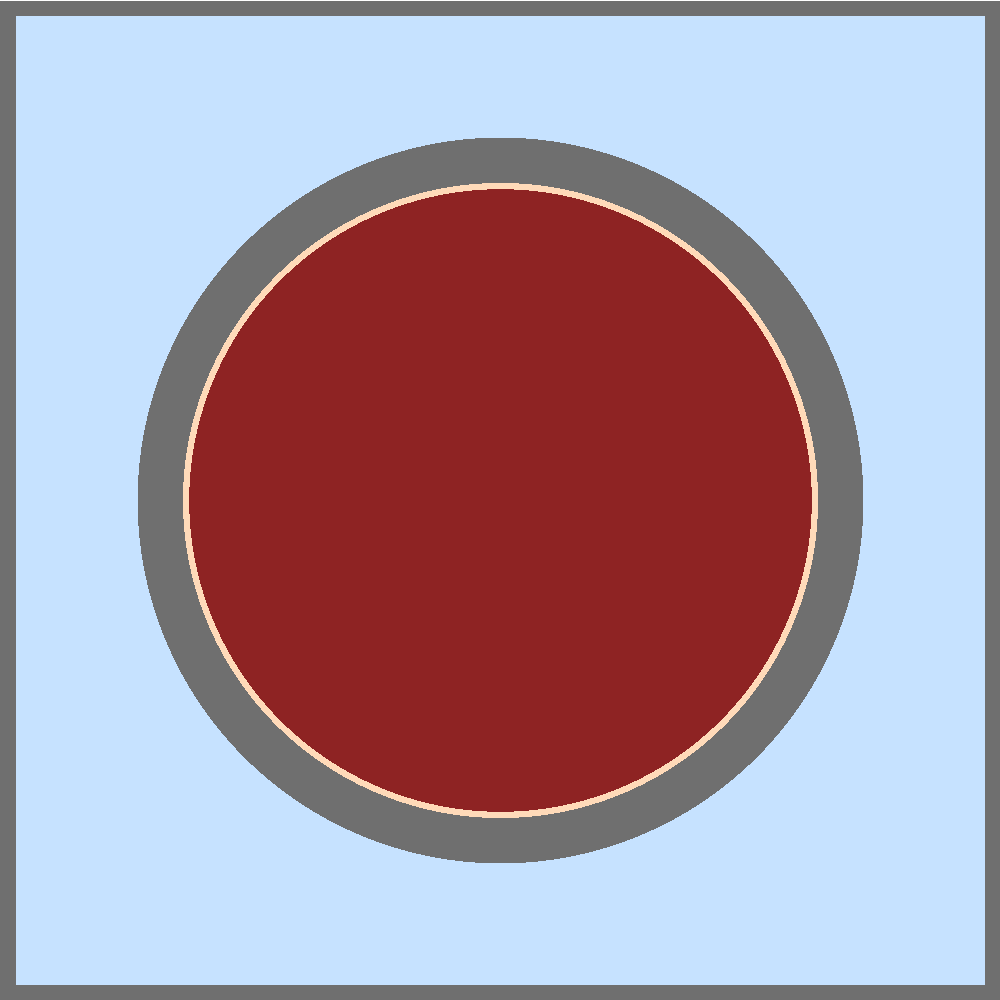
\includegraphics[width=0.9\linewidth]{figures/benchmarks/fuel-pin-16}
  \caption{}
  \label{fig:chap7-pin-1.6}
\end{subfigure}%
\begin{subfigure}{.5\textwidth}
  \centering
  
\includegraphics[width=0.9\linewidth]{figures/benchmarks/guide-tube}
  \caption{}
  \label{fig:chap7-pin-crgt}
\end{subfigure}
\begin{subfigure}{.5\textwidth}
  \centering
  
\includegraphics[width=0.9\linewidth]{figures/benchmarks/instr-tube}
  \caption{}
  \label{fig:chap7-instr-tube}
\end{subfigure}%
\begin{subfigure}{.5\textwidth}
  \centering
  
\includegraphics[width=0.9\linewidth]{figures/benchmarks/burn-abs}
  \caption{}
  \label{fig:chap7-bp}
\end{subfigure}%
\caption[BEAVRS pin cell geometries]{1.6\% enriched fuel pin (a), control rod guide tube (b), instrument tube (c) and burnable poison (d). Light blue is borated water, red is UO$_2$ fuel, gray is zircaloy, brown is helium, white is air and green is borosolicate glass.}
\label{fig:chap7-pin-cells}
\end{figure}

%The radii for each material zone in the pin cells are detailed in Tab.~\ref{table:chap7-pin-cell-radii}. Each pin is surrounded by borated water and a zircaloy egg-crate grid spacer.  The pin cell pitch is 1.25984 cm and the thickness of the grid spacer is 0.02014 cm.

%\addtocounter{footnote}{-2}
%\stepcounter{footnote}\footnotetext{The control rod guide tube geometry above the dashpot.}
%\stepcounter{footnote}\footnotetext{The burnable poison geometry above the dashpot.}


%%%%%%%%%%%%%%%%%%%%%%%%%%%%
\subsection{Fuel Assemblies}
\label{subsec:chap7-fuel-assms}

%The first three benchmark models are based upon 2D models of individual fuel assemblies extracted from the full core \ac{BEAVRS} model. Each assembly consists of a 17$\times$17 rectilinear array of pin cells with a total height and width of 21.41728 cm. The stainless steel grid sleeve and water separating each fuel assembly in the full core \ac{BEAVRS} model are not included in the individual models of each fuel assembly. The intra-pin egg-crate grid spacer is included in each benchmark model. The assemblies are modeled with reflective \acp{BC} to simulate an infinite repeating lattice of each fuel assembly. 

The first three benchmark models are based upon 2D models of individual fuel assemblies extracted from the full core \ac{BEAVRS} model. Each assembly consists of a 17$\times$17 rectilinear array of pin cells with a total height and width of 21.41728 cm. The intra-pin egg-crate grid spacer and grid sleeve separating each fuel assembly in the full core \ac{BEAVRS} model are not included in the individual models of each fuel assembly. The assemblies are modeled with reflective \acp{BC} to simulate an infinite repeating lattice of each fuel assembly. 

\begin{figure}[h!]
  \centering
  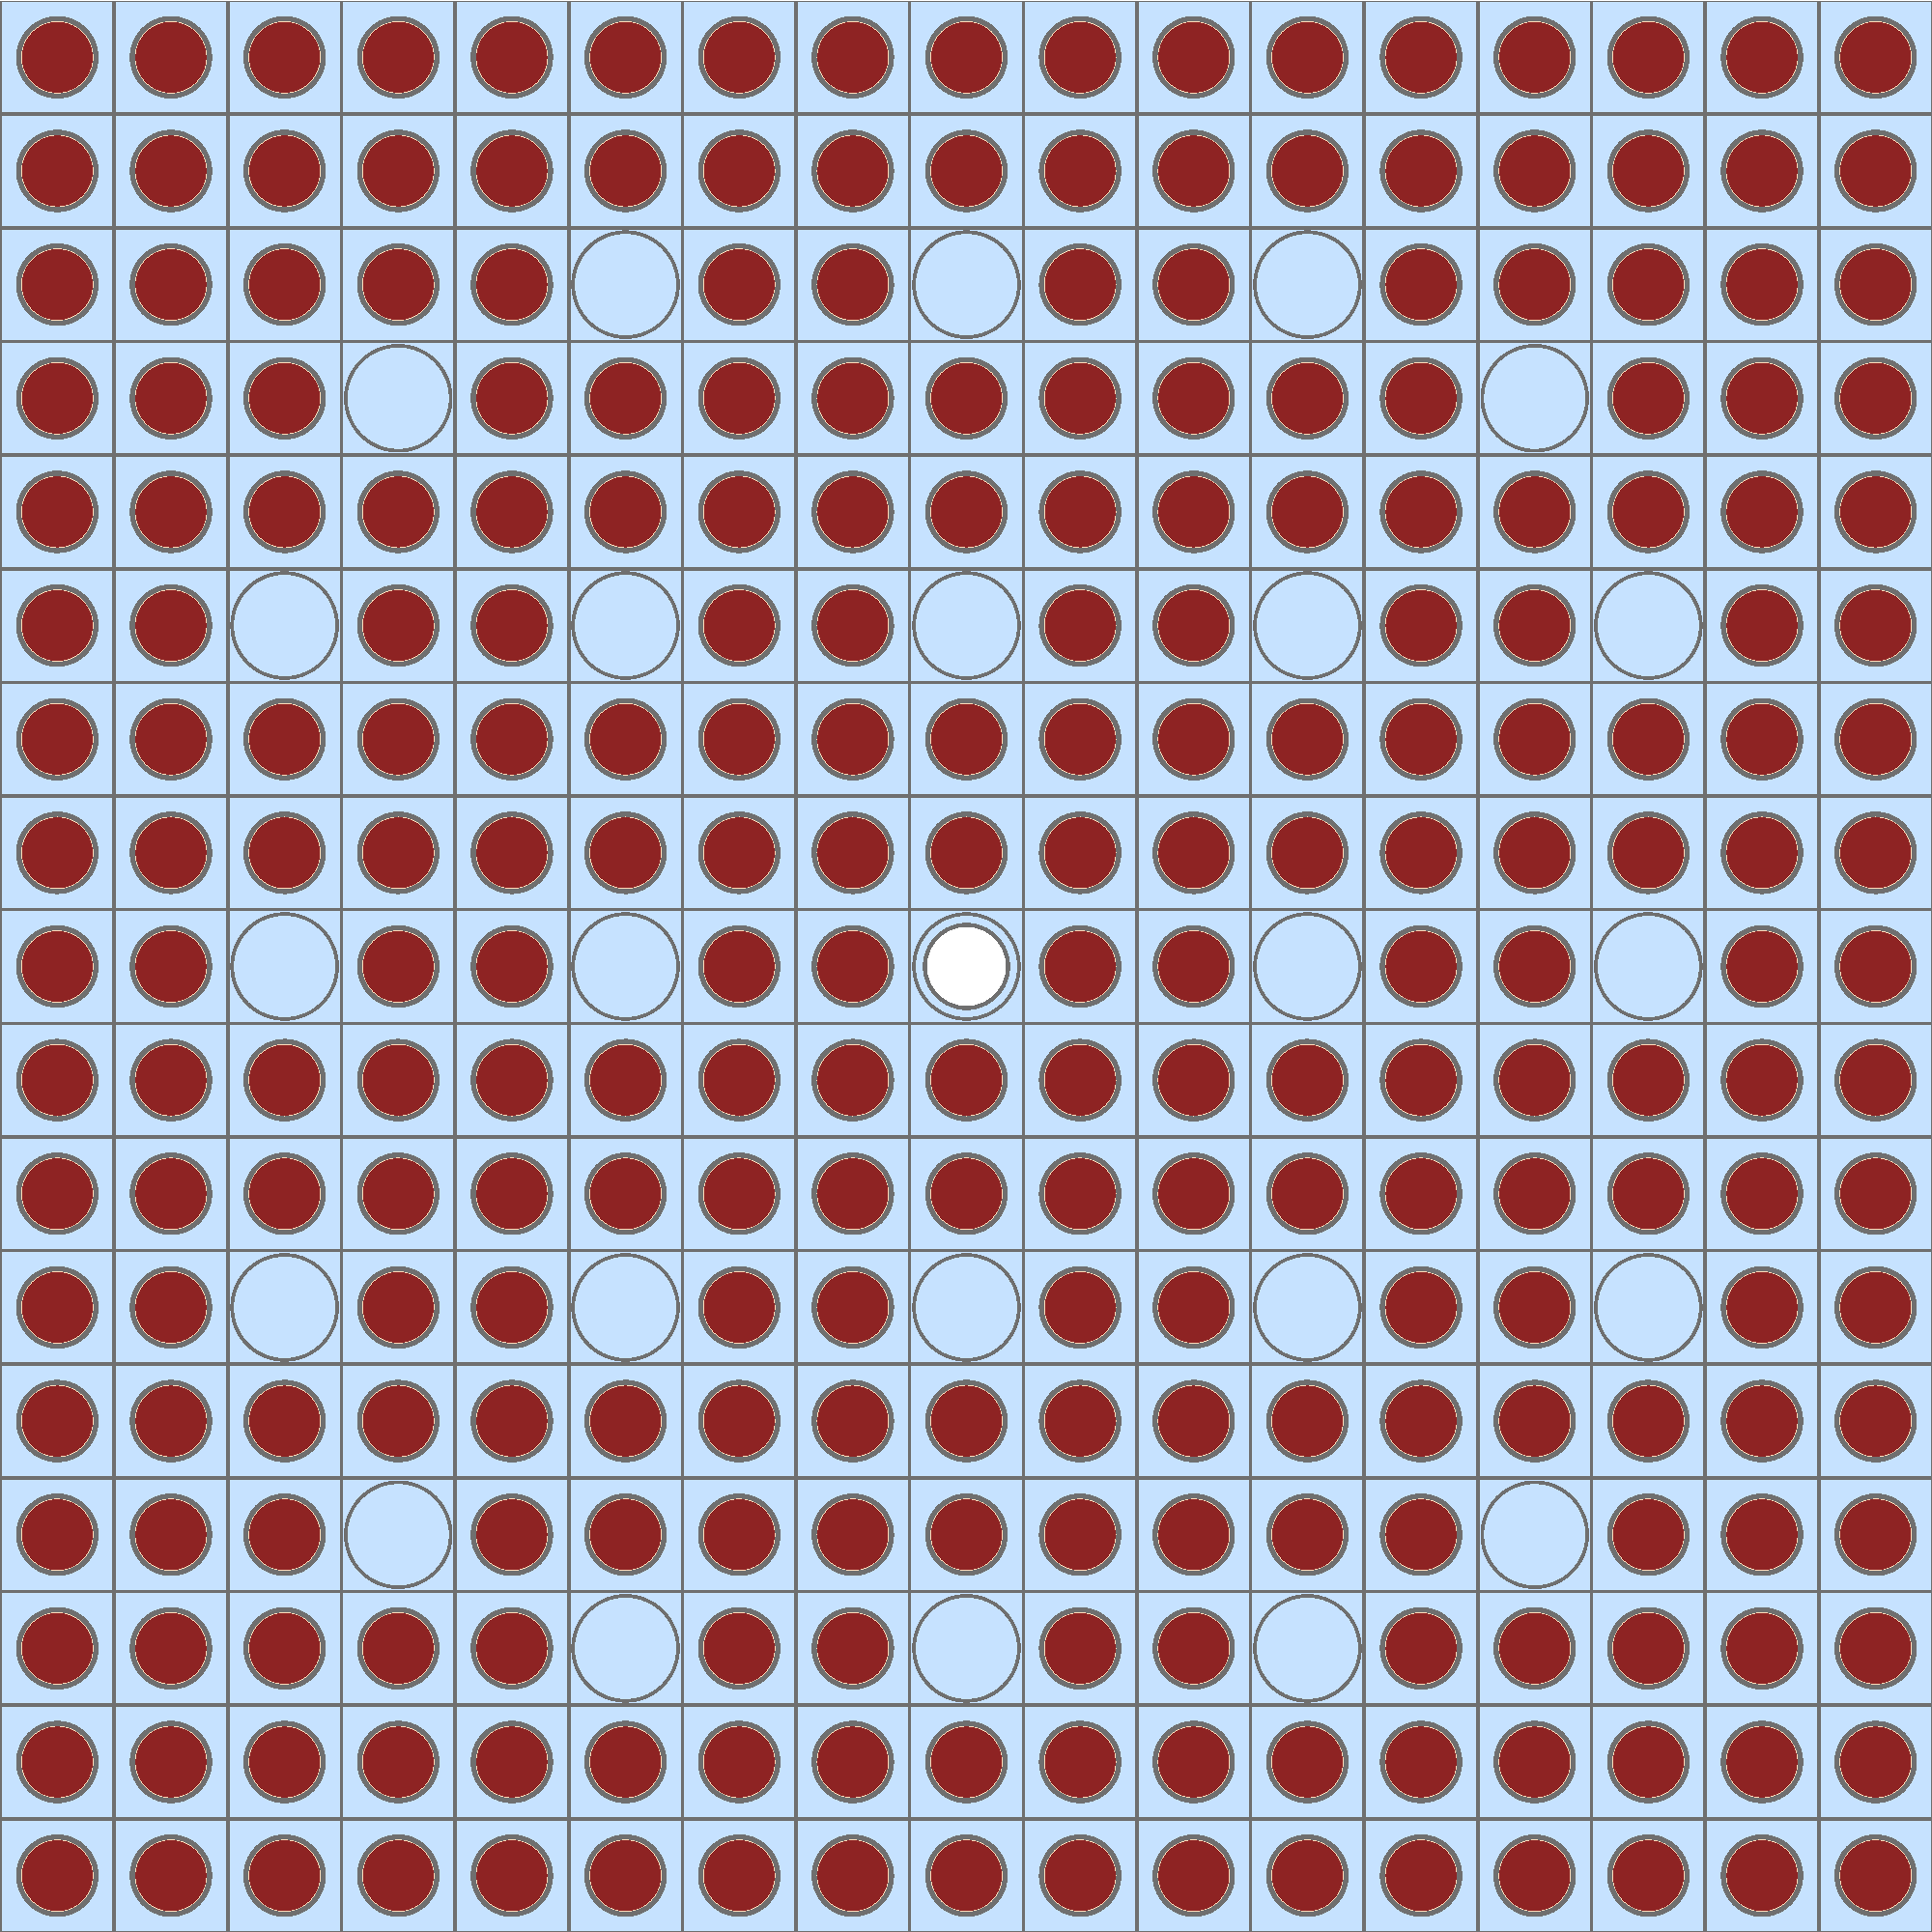
\includegraphics[width=0.65\linewidth]{figures/benchmarks/assembly-16}
\vspace{2mm}
\caption[BEAVRS 1.6\% enriched assembly]{A 1.6\% enriched UO$_2$ fuel assembly without \acp{BP}.}
\label{fig:chap7-assm-16}
\end{figure}

\begin{figure}[h!]
  \centering
  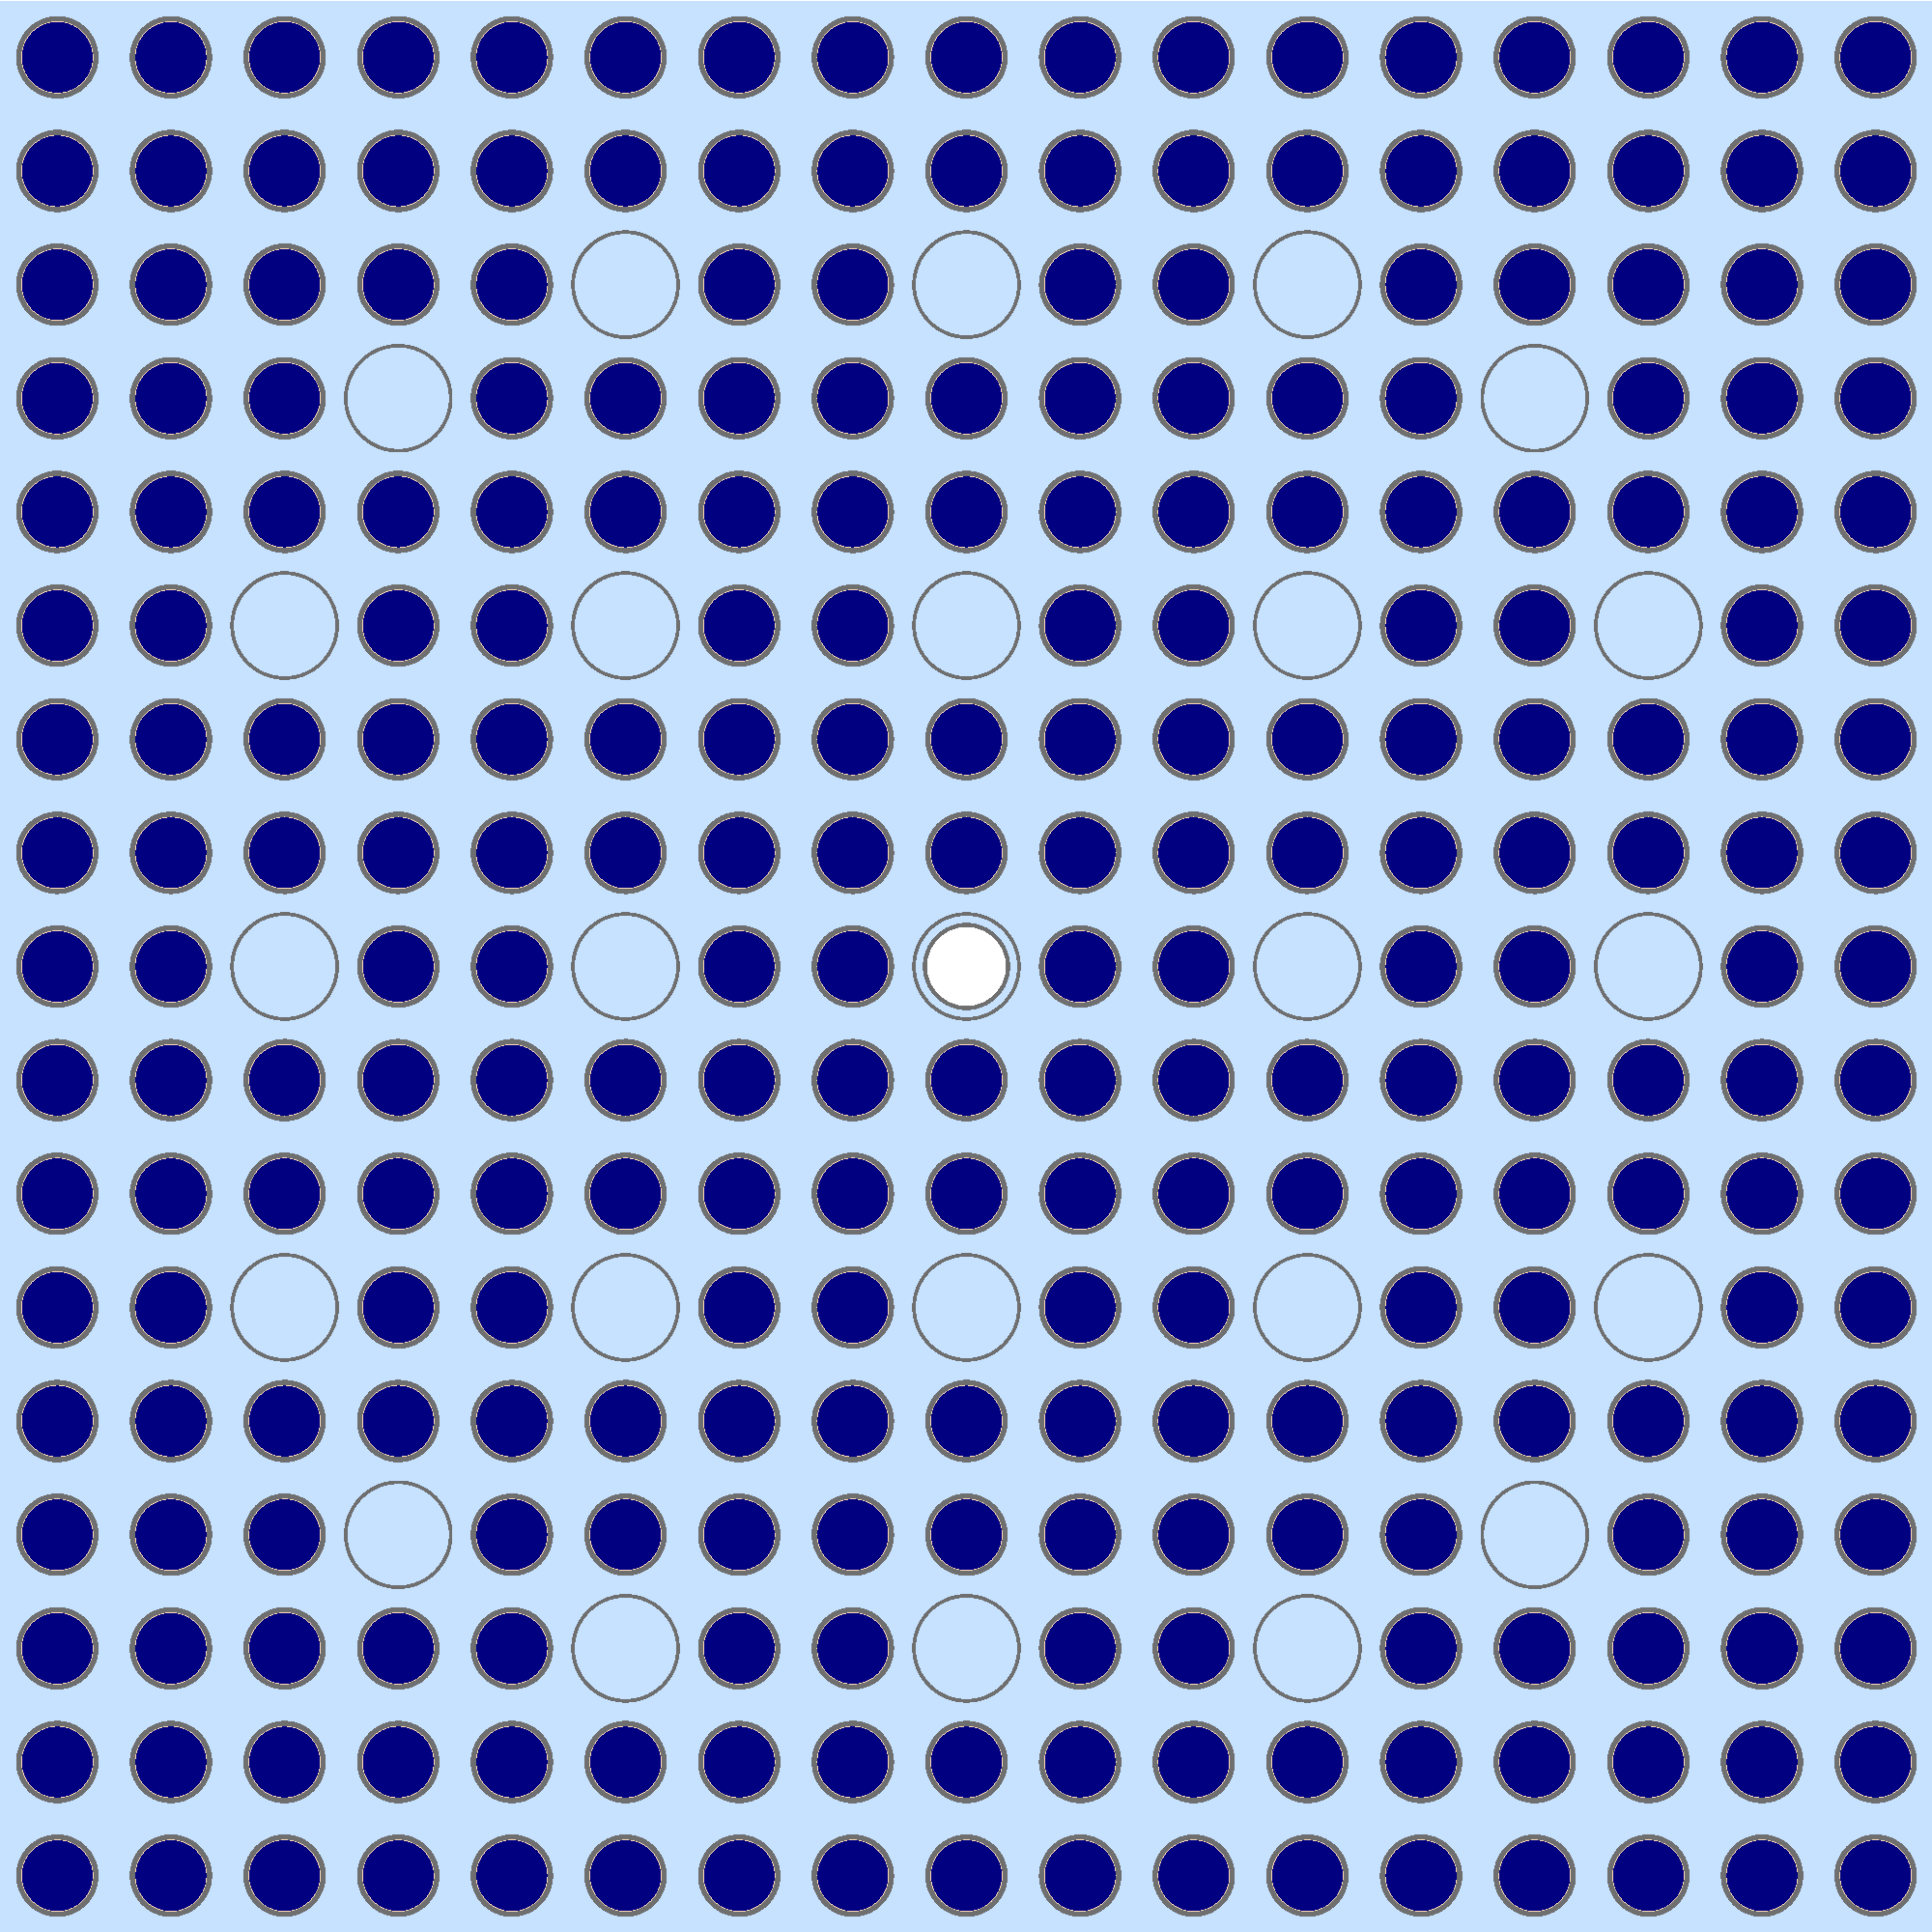
\includegraphics[width=0.65\linewidth]{figures/benchmarks/assembly-31}
\vspace{2mm}
\caption[BEAVRS 3.1\% enriched assembly]{A 3.1\% enriched UO$_2$ fuel assembly without \acp{BP}.}
\label{fig:chap7-assm-31}
\end{figure}

\begin{figure}[h!]
  \centering
  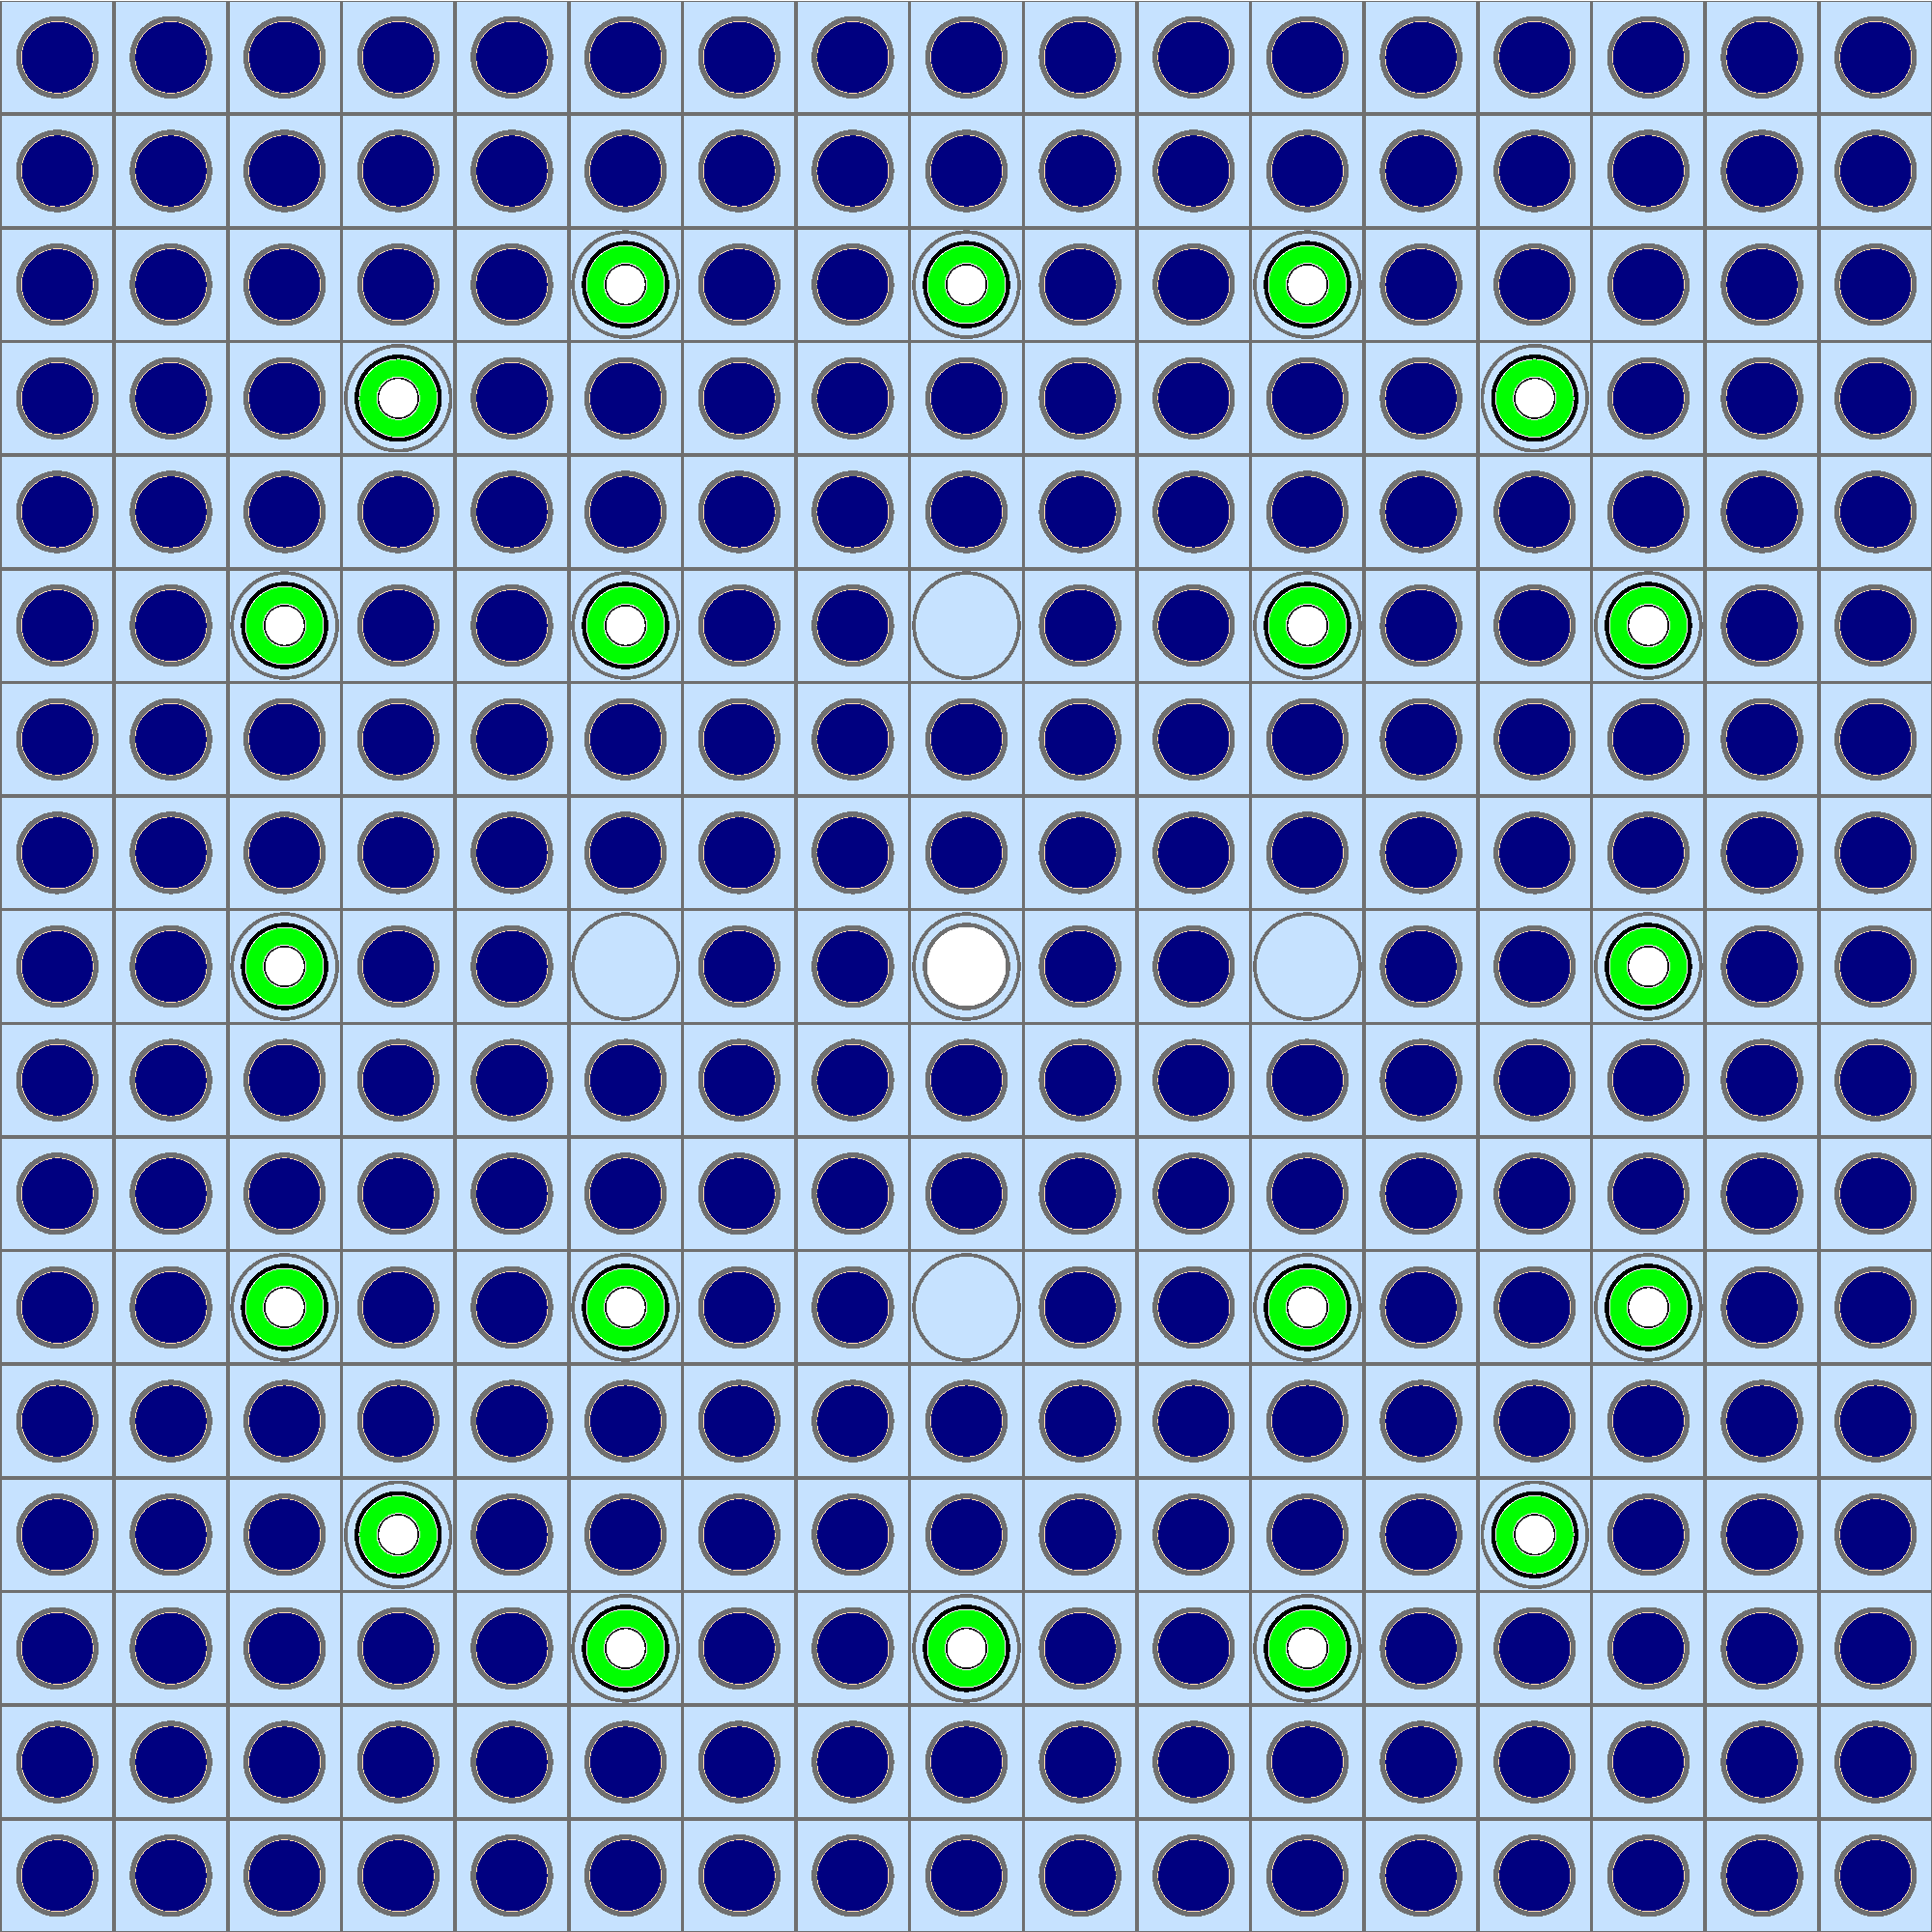
\includegraphics[width=0.65\linewidth]{figures/benchmarks/assembly-31-20BPs}
\vspace{2mm}
\caption[BEAVRS 3.1\% enriched assembly with 20 BPs]{A 3.1\% enriched UO$_2$ fuel assembly with 20 \acp{BP}.}
\label{fig:chap7-assm-31-20BPs}
\end{figure}

The sequence of fuel assembly benchmarks are designed to investigate the impact of fuel enrichment, \acp{CRGT} and \acp{BP} on spatially self-shielded \ac{MGXS}. The first fuel assembly benchmark depicted in Fig.~\ref{fig:chap7-assm-16} consists of 264 fuel pins with 1.6\% enriched UO$_2$ fuel, 24 \acp{CRGT}, and a single central instrument tube. The second benchmark shown in Fig.~\ref{fig:chap7-assm-31} is of the same geometric configuration, but is composed of 3.1\% enriched UO$_2$ fuel. The third benchmark illustrated in Fig.~\ref{fig:chap7-assm-31-20BPs} includes 3.1\% enriched UO$_2$ fuel with a mixture of 20 \acp{BP}, 4 \acp{CRGT} and a single central instrument tube. Although the \ac{BEAVRS} model is composed of assemblies with many different \ac{BP} configurations, only a single assembly with \acp{BP} was studied for practical reasons.

%%%%%%%%%%%%%%%%%%%%%%%%%%%%%%%%%%%%%%
\subsection{2$\times$2 Assembly Colorsets}
\label{subsec:chap7-2x2-colorsets}

%Two benchmarks were constructed from 2$\times$2 colorsets of fuel assemblies from the \ac{BEAVRS} model presented in Sec.~\ref{subsec:chap7-fuel-assms}. The pitch between fuel assemblies in the colorsets is 21.41728 cm (the height/width of each assembly). The stainless steel grid sleeve and water separating each fuel assembly in the full core \ac{BEAVRS} model are not included in the 2$\times$2 colorsets. The intra-pin egg-crate grid spacer is included in each benchmark model. The first colorset is modeled with periodic \acp{BC} on all sides to simulate an infinitely repeating lattice of fuel assemblies. The second colorset is surrounded by a water reflector on the bottom and right that is of the same width as a fuel assembly. The reflected colorset does not include the stainless steel baffle surrounding the fuel assemblies adjacent to the water reflector in the full core \ac{BEAVRS} model. The reflected colorset includes reflective \acp{BC} on the top and left (adjacent to the fuel assemblies) with vacuum \acp{BC} on the bottom and right (adjacent to the reflector).

Two benchmarks were constructed from 2$\times$2 colorsets of fuel assemblies from the \ac{BEAVRS} model presented in Sec.~\ref{subsec:chap7-fuel-assms}. The pitch between fuel assemblies in the colorsets is 21.41728 cm (the height/width of each assembly). The intra-pin egg-crate grid spacer and grid sleeve separating each fuel assembly in the full core \ac{BEAVRS} model are not included in the 2$\times$2 colorsets. The first colorset is modeled with periodic \acp{BC} on all sides to simulate an infinitely repeating lattice of fuel assemblies. The second colorset is surrounded by a water reflector on the bottom and right that is of the same width as a fuel assembly. The reflected colorset does not include the stainless steel baffle surrounding the fuel assemblies adjacent to the water reflector in the full core \ac{BEAVRS} model. The reflected colorset includes reflective \acp{BC} on the top and left (adjacent to the fuel assemblies) with vacuum \acp{BC} on the bottom and right (adjacent to the reflector).

\begin{figure}[h!]
  \centering
  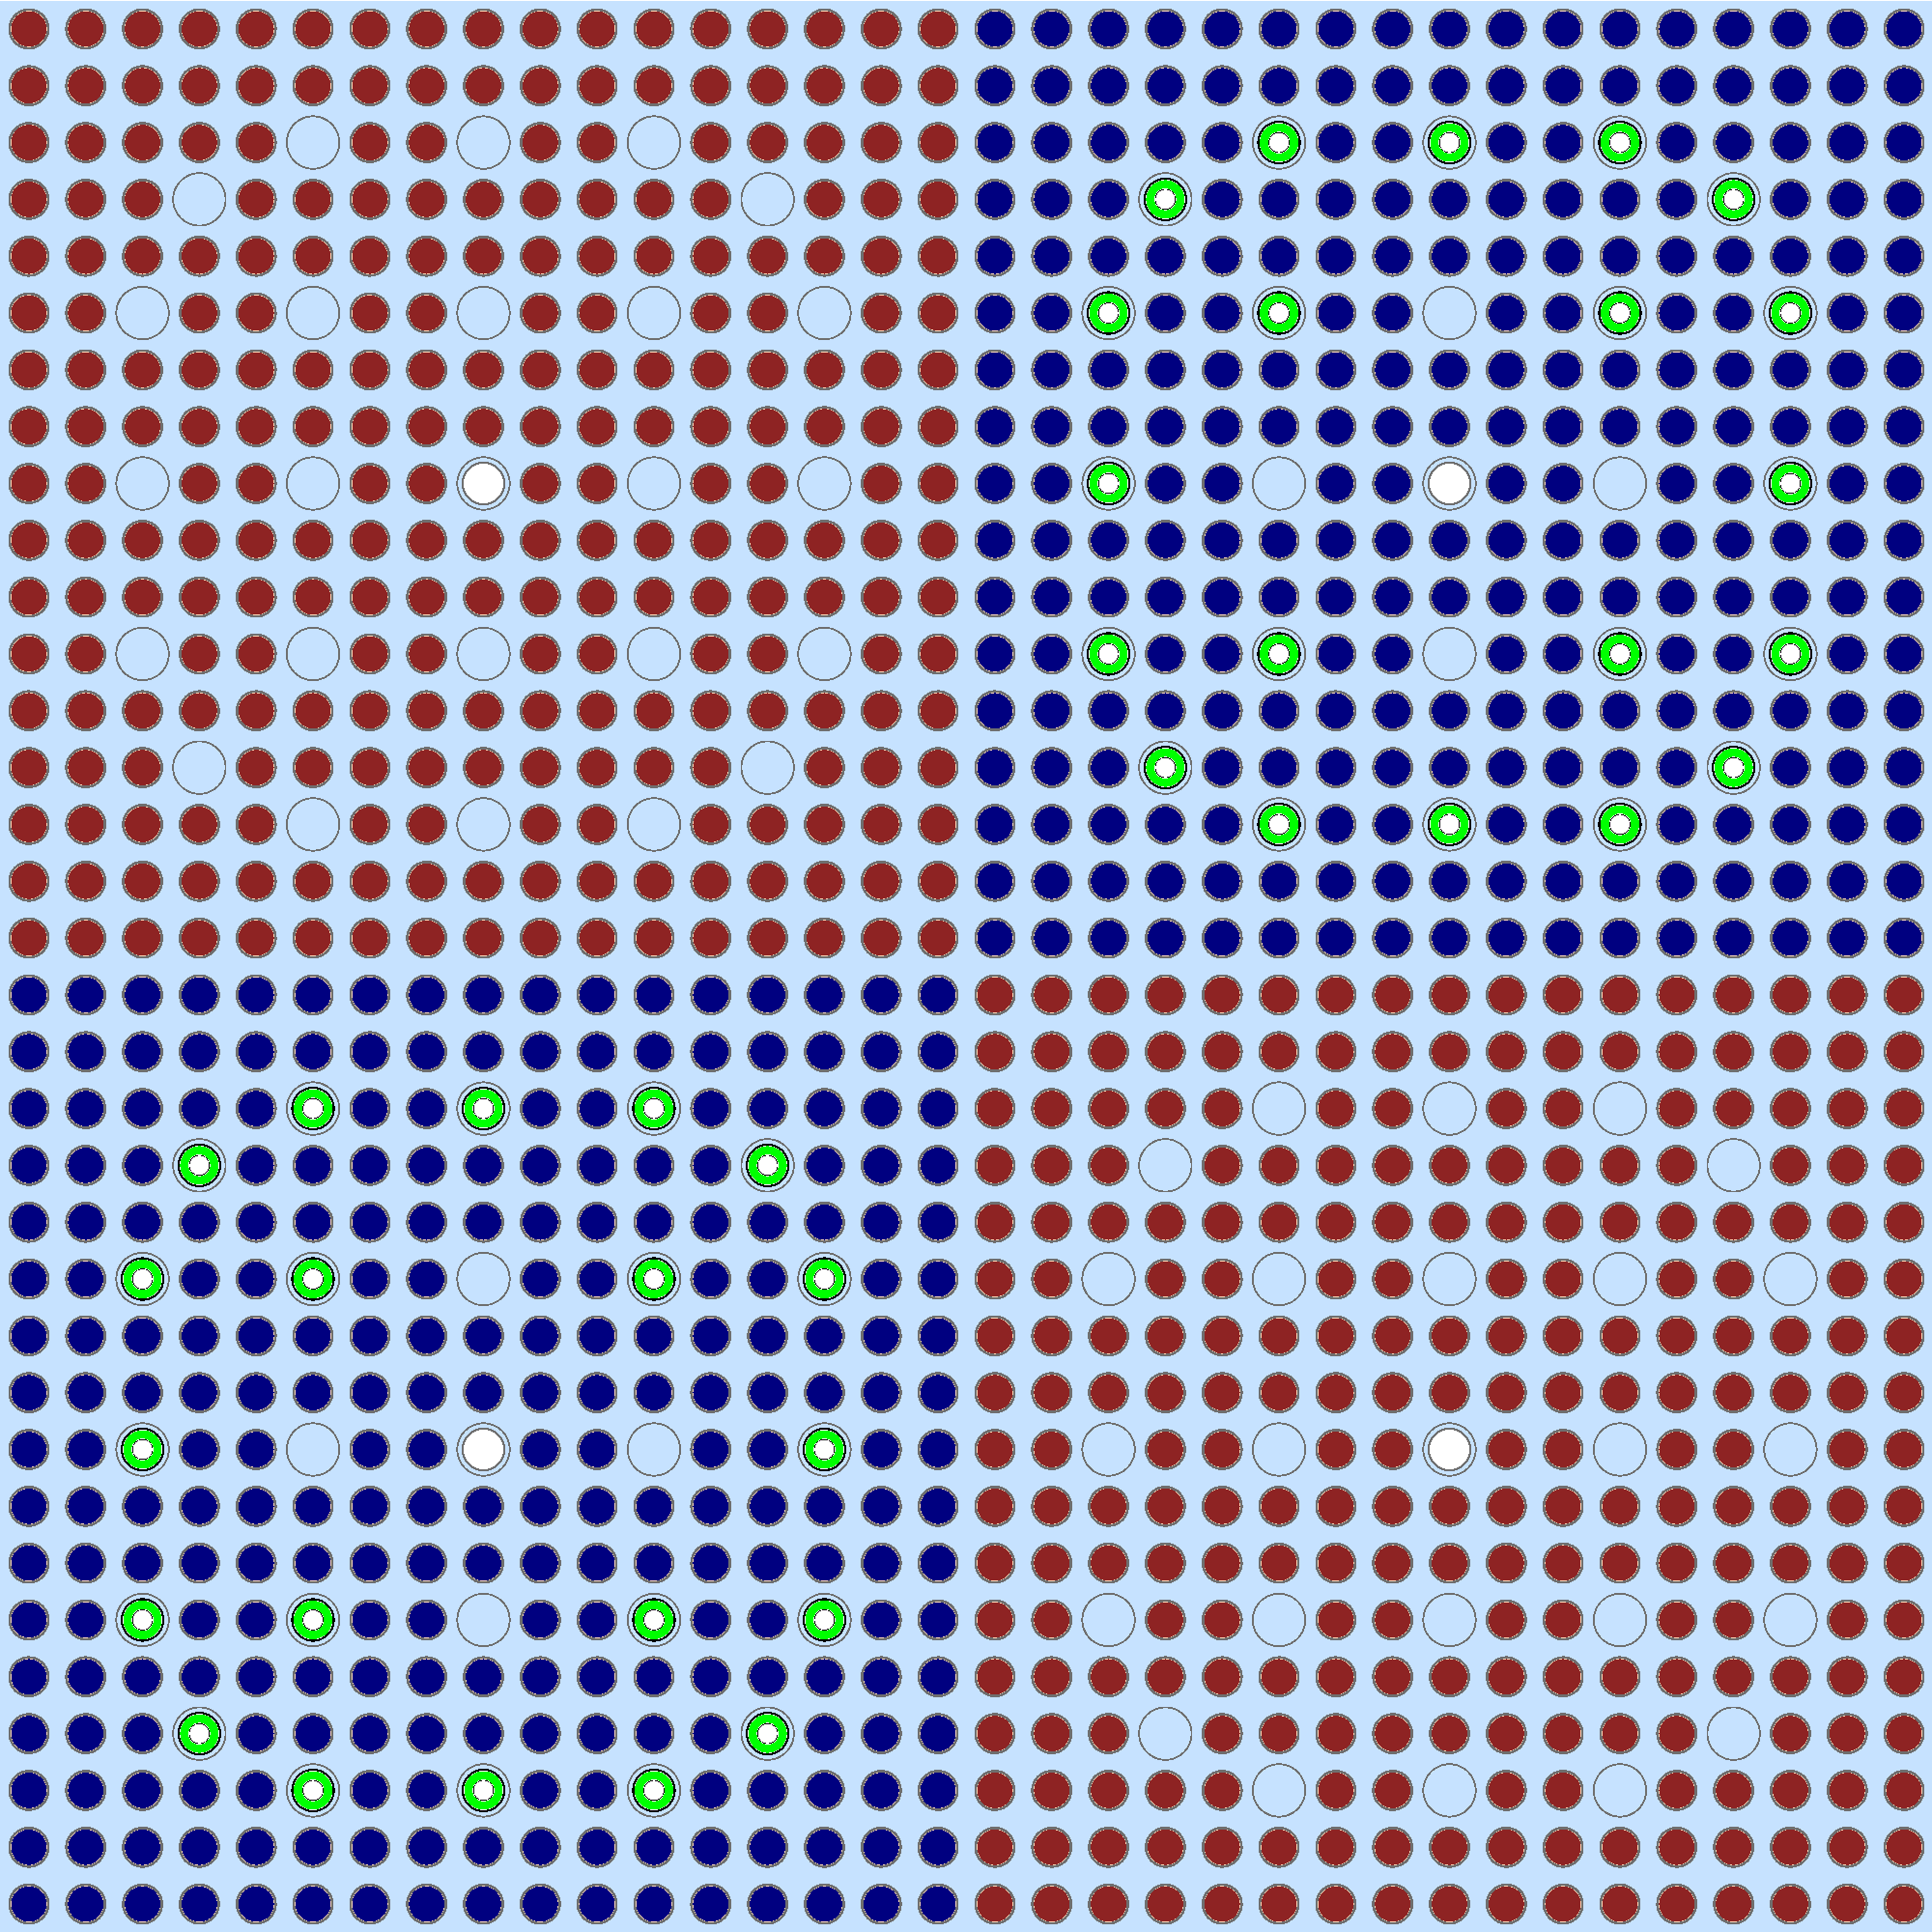
\includegraphics[width=0.63\linewidth]{figures/benchmarks/2x2}
\vspace{2mm}
\caption[A 2$\times$2 colorset of BEAVRS assemblies]{A 2$\times$2 colorset of BEAVRS assemblies with periodic BCs.}
\label{fig:chap7-2x2}
\end{figure}

\begin{figure}[h!]
  \centering
  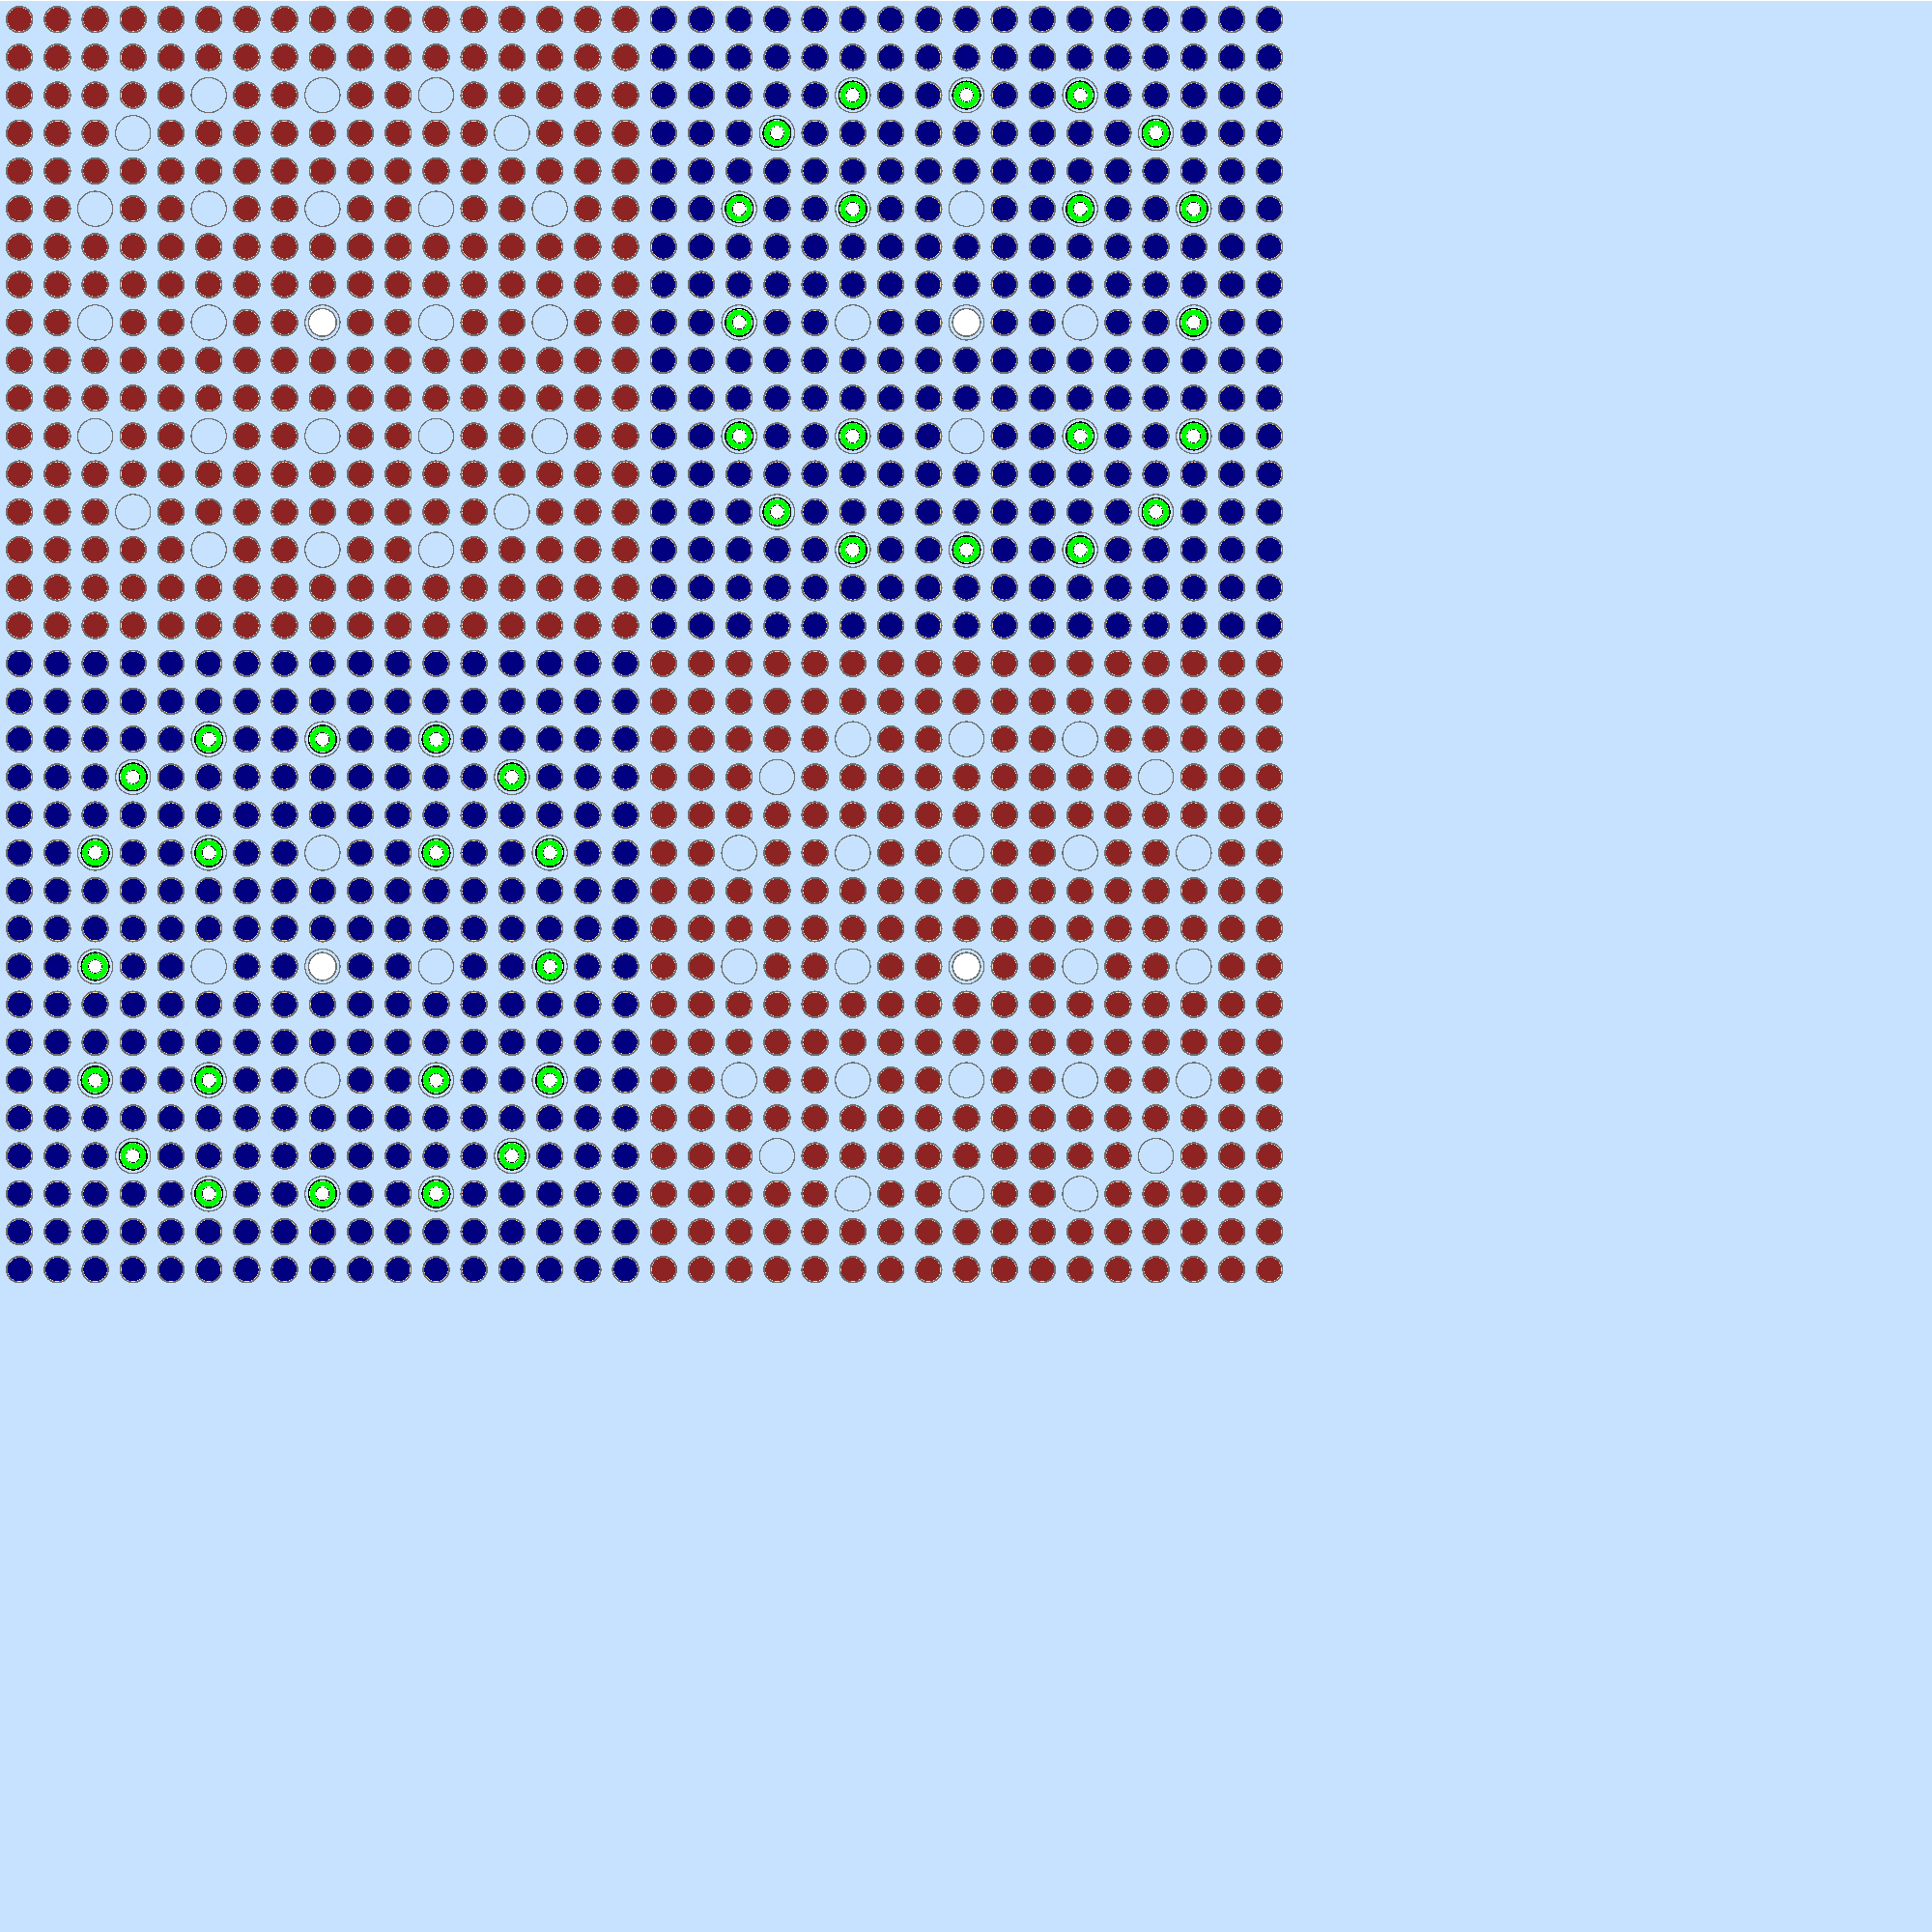
\includegraphics[width=0.63\linewidth]{figures/benchmarks/reflector}
\vspace{2mm}
\caption[A reflected 2$\times$2 colorset of BEAVRS assemblies]{A 2$\times$2 colorset of BEAVRS assemblies surrounded by a water reflector. Reflective \acp{BC} were applied on the left/top, with vacuum \acp{BC} on the right/bottom.}
\label{fig:chap7-reflector}
\end{figure}

The first 2$\times$2 colorset model shown in Fig.~\ref{fig:chap7-2x2} is composed of a checkerboard pattern of the fuel assemblies of 1.6\% enriched UO$_2$ without \acp{BP} (Fig.~\ref{fig:chap7-assm-16}) and 3.1\% enriched UO$_2$ with 20 \acp{BP} (Fig.~\ref{fig:chap7-assm-31-20BPs}). The first colorset benchmark is designed to investigate the effects of inter-assembly spatial heterogeneities on the spatially self-shielded \ac{MGXS} of fuel pins of different enrichments (\textit{i.e.}, from different fuel assemblies) placed adjacent to one another. The second benchmark illustrated in Fig.~\ref{fig:chap7-reflector} is the same 2$\times$2 colorset of fuel assemblies, but is surrounded by a water reflector. This benchmark is designed to quantify the impact of the moderation provided by the reflector, as well as the leakage of neutrons through the reflector, on spatially self-shielded \ac{MGXS}.

%%%%%%%%%%%%%%%%%%%%%%%%%%%%%
\subsection{BEAVRS Quarter Core}
\label{subsec:chap7-full-core}

The sixth and final benchmark is a 2D planar slice of the top right quadrant of the quadrant symmetric \ac{BEAVRS} core model\footnote{The \ac{BEAVRS} model was made quadrant symmetric by replacing all instrument tubes with empty \acp{CRGT}.} at the axial mid-plane as shown in Fig.~\ref{fig:chap7-full-core}. The fuel assemblies in the model are configured according to the cycle 1 loading pattern detailed in the \ac{BEAVRS} specifications~\cite{horelik2013beavrs}. The quarter core model includes assemblies with 1.6\%, 2.4\% and 3.1\% enriched UO$_2$ fuel depicted as red, blue and yellow in Fig.~\ref{fig:chap7-full-core}, respectively. The benchmark model is the all rods out configuration with a critical boron concentration of 975 ppm~\cite{horelik2013beavrs}.

The intra-pin egg-crate grid spacer and grid sleeve separating each fuel assembly in the 3D core \ac{BEAVRS} model are not included in 2D model at the axial mid-plane. All other radial heterogeneities in the \ac{BEAVRS} specifications are included in this model, including the inter-assembly water gaps, stainless steel baffle surrounding the fuel assemblies, core barrel, neutron shield panels and pressure vessel. The space outside of the pressure vessel is filled with air with vacuum \acp{BC} applied to planar surfaces on the top, bottom, left and right. The 2D quarter core \ac{BEAVRS} model builds upon the preceding five simpler benchmarks to explore the impact of radial heterogeneities in a realistic core configuration on spatially self-shielded \ac{MGXS}.

\begin{figure}[h!]
  \centering
  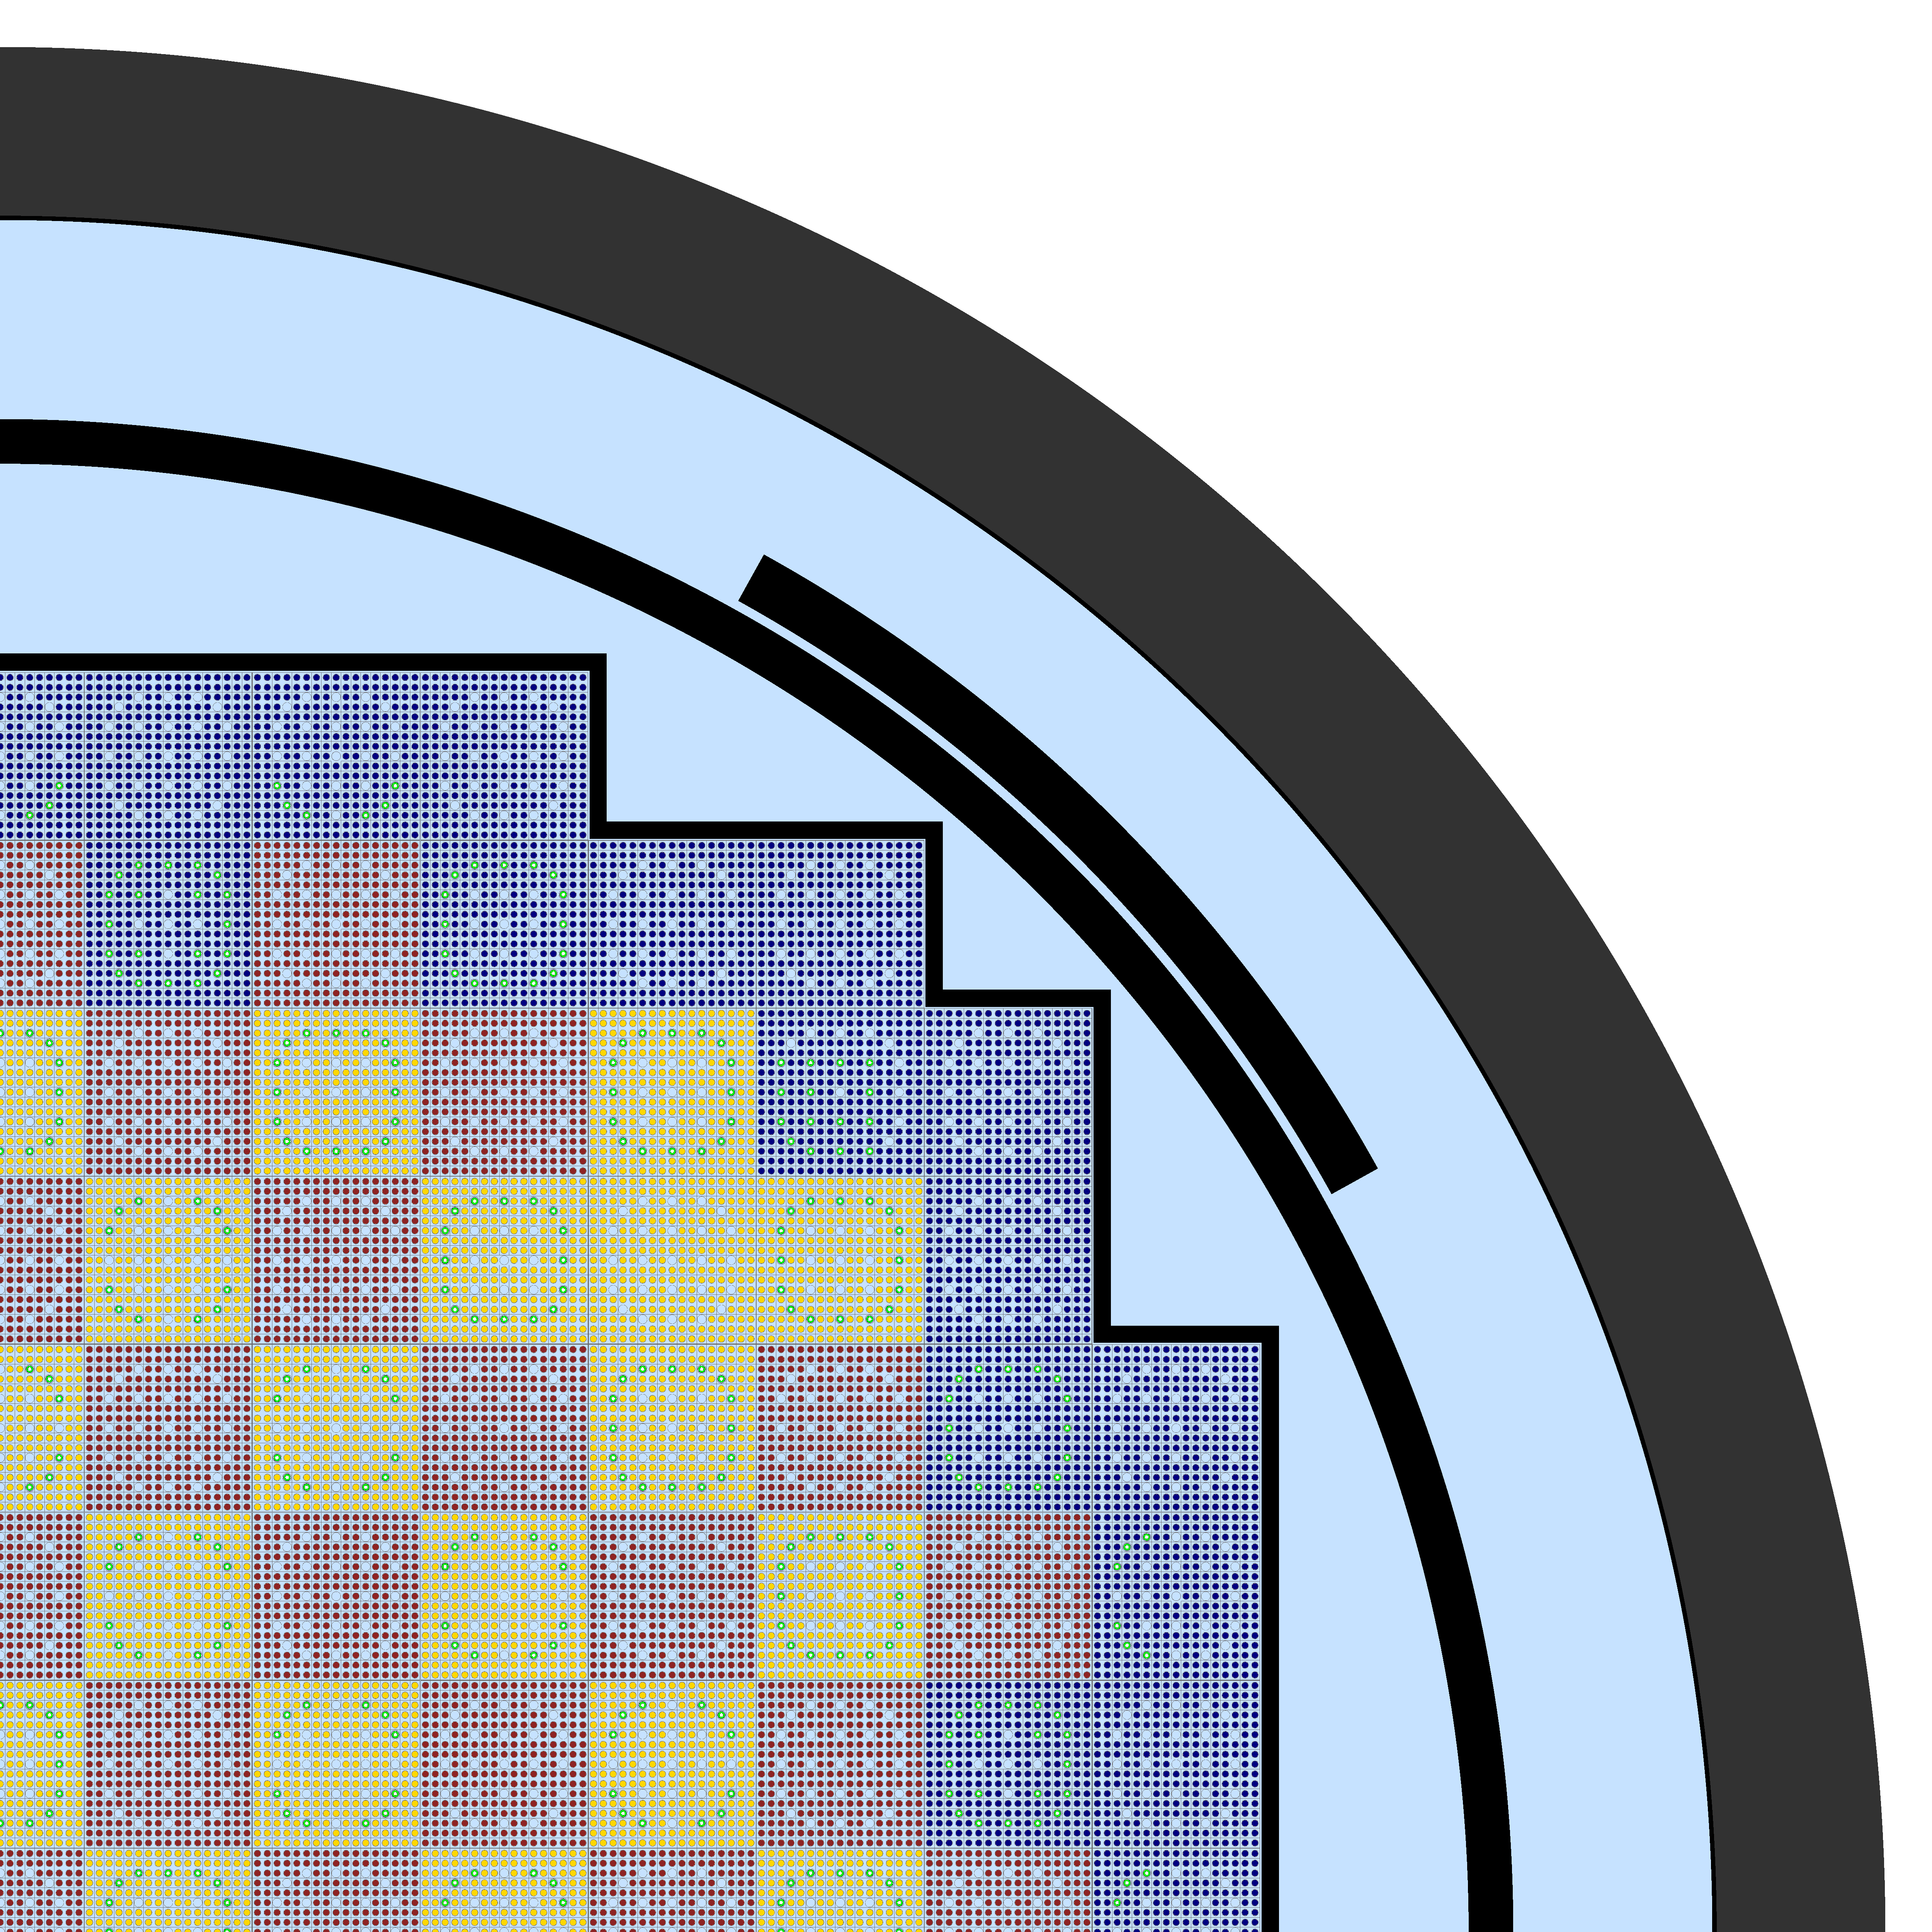
\includegraphics[width=0.9\linewidth]{figures/benchmarks/quarter-core}
\vspace{2mm}
\caption[The 2D quarter core \ac{BEAVRS} model]{The 2D quarter core \ac{BEAVRS} model.}
\label{fig:chap7-full-core}
\end{figure}


%%%%%%%%%%%%%%%%%%%%%%%%%%%%%%%%%%%%%%%%%%%%%%%%%%%%%%%%%%%%%%%%%%%%%%%%%%%%%%%
\section{Reference Results}
\label{sec:chap7-ref-results}

This section presents the reference results computed using OpenMC for each of the six benchmarks presented in the preceding section. As discussed in Sec.~\ref{subsec:chap7-src-stationarity}, OpenMC was employed to compute the Shannon entropy to determine the number of batches of particle histories needed to reach source stationarity. Sec.~\ref{subsec:chap7-eigenvalues} presents the converged $k_{eff}$ eigenvalue computed by OpenMC for each of the six benchmarks. Finally, Sec.~\ref{subsec:chap7-pin-powers} and Sec.~\ref{subsec:chap7-capture-rates} present the reference pin-wise spatial distributions of fission rates and U-238 capture rates in each benchmark as tallied in OpenMC along with their associated statistical uncertainties.

The ENDF/B-VII.1 continuous energy cross section libraries evaluated at 600K provided by the MCNP code~\cite{mcnpx2003manual} were used by OpenMC for all simulations. It should be noted that isotropic in lab scattering was employed for all reference calculations with OpenMC's iso-in-lab feature (see Sec.~\ref{subsec:chap4-iso-in-lab}). Although isotropic in lab scattering is a poor approximation for \acp{LWR}, it eliminated scattering source anisotropy as one possible cause of approximation error between OpenMC and OpenMOC\footnote{At the time of this writing, OpenMOC employed an isotropic in lab neutron scattering kernel.} in order to isolate approximation errors resulting from spatially self-shielded \ac{MGXS}.

The reference solutions for each assembly and colorset benchmark model was computed with 100 inactive and 900 active batches of 10$^7$ particle histories per batch. The reference solution for the quarter core \ac{BEAVRS} model was computed with 200 inactive and 800 active batches of 10$^8$ histories per batch. Each OpenMC simulation was performed in parallel on ten compute nodes on the Falcon supercomputer at Idaho National Laboratory. Each compute node contained two dual socket Intel Xeon E5-2680 CPUs with 12 cores and 132 gigabytes of DRAM\footnote{Dynamic Random Access Memory.}. Four MPI processes were launched on each node (two MPI processes per CPU) with 6 OpenMP parallel threads per MPI process.

%%%%%%%%%%%%%%%%%%%%%%%%%%%%%%%
\subsection{Source Stationarity}
\label{subsec:chap7-src-stationarity}

The first metric that was evaluated for each of the six benchmarks was the stationarity of the fission source distribution. The initial distribution of fission source sites is uniformly distributed in space across fissile material zones by OpenMC for the first batch of particle histories. Each subsequent batch of fission source sites is drawn from a bank of fission sites populated during the preceding batch of particle histories. In eigenvalue calculations, the distribution of fission source sites must reach stationarity before tallying integral quantities such as the eigenvalue or reaction rates. 

The Shannon entropy is a commonly used diagnostic to measure source stationarity in \ac{MC} eigenvalue calculations~\cite{brown2006entropy}. To compute the Shannon entropy, a mesh of $M$ mesh cells is superimposed across the geometry and the number of fission source cites in each mesh cell is tabulated. The empirical multinomial probabilities $p_{i}$ for fission source sites is computed for each mesh cell $i$ as the ratio of sites in that cell to the total number of source sites in the geometry. The Shannon entropy $H$ is then computed from the multinomial probability distribution from the following equation:

\begin{equation}
\label{eqn:chap7-shannon-entropy}
H = \displaystyle\sum\limits_{i=1}^{M} p_{i} \log_{2} p_{i}
\end{equation}

\noindent The Shannon entropy provides a single scalar value which characterizes the spatial distribution of fission source sites. By monitoring the value of $H$ for each batch, one may determine the number of inactive batches needed to reach source stationarity.

The Shannon entropy was computed using a rectilinear pin-wise mesh for each of the six benchmark models and plotted in Fig.~\ref{fig:chap7-entropy}. The entropies in the plot are normalized to the entropy at the final 1000$^{\text{th}}$ batch in order to standardize the entropies for comparison in the same plot. The entropies for each of the three fuel assembly benchmarks, as well as the 2$\times$2 colorset without a reflector, all lie very near unity and do not exhibit any convergence behavior in the plot. The entropy for the 2$\times$2 colorset with a reflector appears to converge to near unity within 30 batches. Finally, the entropy for the high dominance ratio \ac{BEAVRS} quarter core appears to converge within 200 batches. 

\begin{figure}[h!]
  \centering
  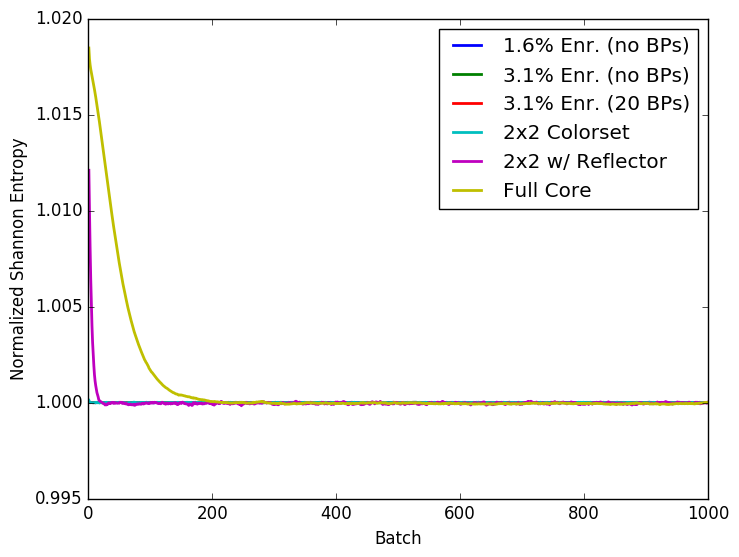
\includegraphics[width=0.7\linewidth]{figures/benchmarks/entropy/entropy-all}
\caption[Shannon entropy source convergence for BEAVRS geometries]{Shannon entropy source convergence for BEAVRS geometries.}
\label{fig:chap7-entropy}
\end{figure}

As expected, the number of batches required to reach source stationarity increases with the benchmark size and heterogeneity, and the corresponding increase in the dominance ratio. This analysis of the Shannon entropy for each benchmark was used to determine an appropriately conservative number of inactive batches to employ in all subsequent OpenMC simulations of each benchmark model. In particular, all OpenMC simulations of the single assembly and 2$\times$2 colorsets use 100 inactive batches prior to tallying the eigenvalue, reference reaction rate distributions and \ac{MGXS}. Similarly, 200 inactive batches are used for the quarter core \ac{BEAVRS} model.

%%%%%%%%%%%%%%%%%%%%%%%%
\subsection{Eigenvalues}
\label{subsec:chap7-eigenvalues}

The reference eigenvalues were computed for each of the six benchmarks and are listed in Tab.~\ref{table:chap7-ref-eigenvalues}. The OpenMC ``combined'' eigenvalue estimator is reported along with the associated one sigma uncertainty of 1 \ac{pcm} or less for each of the benchmarks. The total runtimes required for the OpenMC simulations to generate the reference eigenvalues are also reported in the table. 

%A total of 9,000,000,000 particle histories (900 active batches of 10$^7$ particle histories per batch) were simulated for the individual fuel assembly and 2$\times$2 colorset benchmarks, while 8,000,000,000 total particle histories (800 active batches) were simulated for the quarter core \ac{BEAVRS} model.

\begin{table}[h!]
  \centering
  \caption[Reference $k^{OpenMC}_{eff}$ for heterogeneous benchmarks]{Reference $k^{OpenMC}_{eff}$ for heterogeneous benchmarks.}
  \small
  \label{table:chap7-ref-eigenvalues}
  \vspace{6pt}
  \begin{tabular}{l C{4cm} r}
  \toprule
  \rowcolor{lightgray}
  \textbf{Benchmark} & $\bm{k^{OpenMC}_{eff}}$ & \textbf{Runtime [core-hours]} \\
  \midrule
  1.6\% Enriched Assembly (no \ac{BP}s) & 0.99326 $\pm$ 0.00001 & 1,005 \\
  3.1\% Enriched Assembly (no \ac{BP}s) & 1.21657 $\pm$ 0.00001 & 891 \\
  3.1\% Enriched Assembly (20 \ac{BP}s) & 1.03315 $\pm$ 0.00001 & 879 \\
  2$\times$2 Colorset & 1.01814 $\pm$ 0.00001 & 903 \\
  2$\times$2 Colorset w/ Reflector & 0.94574 $\pm$ 0.00001 & 895 \\
  \ac{BEAVRS} Quarter Core & 1.02446 $\pm$ 0.00000 & 10,892 \\
  \bottomrule
\end{tabular}
\end{table}

As expected, the eigenvalues increase with enrichment and decrease with the presence of \acp{BP} for the single fuel assembly benchmarks. The eigenvalue for the 2$\times$2 colorset is reduced with the addition of a reflector due to leakage, and to a lesser extent, absorption in the reflector. Although the quarter core \ac{BEAVRS} model is a critical configuration, the eigenvalue is nearly 2500 pcm supercritical due to the iso-in-lab scattering approximation\footnote{An identical OpenMC simulation of the  3D full core \ac{BEAVRS} model using normal anisotropic scattering produced an eigenvalue of 0.99922 $\pm$ 0.00000.}. The eigenvalues reported in Tab.~\ref{table:chap7-ref-eigenvalues} are used to validate the OpenMOC simulations with \ac{MGXS} generated by OpenMC throughout the following chapters.

%%%%%%%%%%%%%%%%%%%%%%%%%%%%%%%%%%%%
\subsection{Fission Rate Spatial Distributions}
\label{subsec:chap7-pin-powers}

The reference energy-integrated fission rate spatial distributions for each of the six benchmarks were computed using rectilinear, pin-wise tally meshes in OpenMC. The fission rates were volume-integrated across each fuel pin and include fission from all nuclides (only U-235 and U-238 for the fresh \ac{PWR} UO$_2$ fuel in the benchmarks). The fission rates were normalized to the mean of all non-zero fission rates in each benchmark. The percent relative errors for the tallied fission rates was computed from the ratio of the sample standard deviation to the mean fission rate in each fuel pin. The fission rates for the quarter core \ac{BEAVRS} model were appropriately tiled to display the equivalent distribution across the quadrant symmetric full core.

The fission rate spatial distributions and percent relative errors for each of the six benchmarks are presented as heatmaps in Figs.~\Crefrange{fig:chap7-fiss-rates-1.6-assm}{fig:chap7-fiss-rates-full-core}. The fission rates in the instrument tubes, \acp{CRGT} and \acp{BP} are all zero and are illustrated in white. The color bars for each of the heatmaps range from the minimum non-zero fission rate to the maximum fission rate for all fuel pins in each benchmark geometry. The statistical error at the final 1000$^{\text{th}}$ batch is less than or equal to 0.5\% for all of the benchmarks. These reference fission rate spatial distributions are used to validate the OpenMOC simulations with \ac{MGXS} generated by OpenMC throughout the following chapters.

%The batch-wise convergence rates of the fission rates is shown for the maximum and mean percent relative errors for each of the benchmarks in Fig.~\ref{fig:chap7-fiss-rates-conv}.

As illustrated in the figures, the fission rate distributions are strongly dependent on the spatially heterogeneous features in each benchmark geometry. For example, the \acp{CRGT} provide additional moderation and increase the fission rates in nearby fuel pins. The presence of \acp{BP} reduces the neutron population and therefore the fission rates for the surrounding fuel pins, while increasing the variation between the minimum and maximum fission rates. The presence of a reflector with a mixture of vacuum and reflective \acp{BC} induces a tilt in the fission rates across the assemblies in the 2$\times$2 colorset, with the maximum fission rates located in the interior fuel pins and the minimum fission rates occurring near the reflector due to neutron leakage. The fission rates for the quarter core \ac{BEAVRS} model in Fig.~\ref{fig:chap7-fiss-rates-full-core} form a highly complex spatial distribution due to the convolution of many different interacting spatial self-shielding effects.

It should be noted that the fission rate distribution for the quarter core \ac{BEAVRS} model is highly skewed due to the isotropic in lab scattering approximation. This can be seen from comparison of Fig.~\ref{fig:chap7-fiss-rate-mean-full-core} with the true fission rate distribution calculated with normal anisotropic scattering in Fig.~\ref{fig:benchmarks-beavrs-fiss-aniso}. The power distribution is highly sensitive to anisotropic scattering due to radial leakage out of the core, and is more peaked near the corner reflectors when the isotropic approximation is made. Although isotropic scattering is unphysical, it allows direct comparisons of OpenMC and OpenMOC results in latter chapters to quantify the impact of various approaches to spatially homogenize \ac{MGXS} without conflicting effects due to the isotropic scattering model used in OpenMOC.

\begin{figure}[h!]
\centering
\begin{subfigure}{0.44\textwidth}
  \centering
  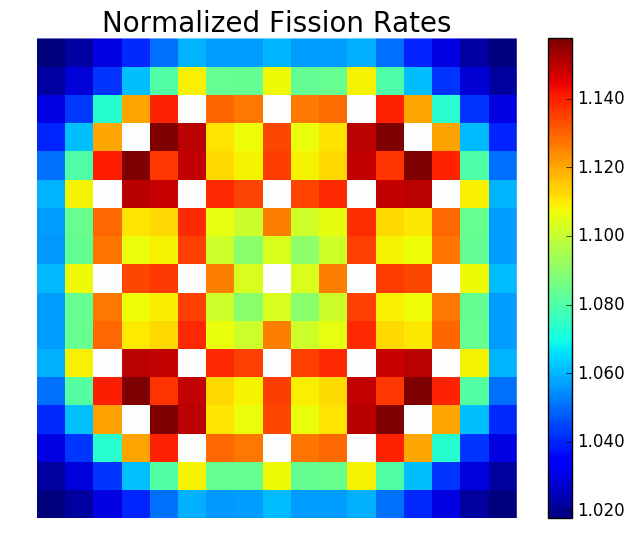
\includegraphics[width=\linewidth]{figures/benchmarks/fission-rates/fiss-mean-assm-16}
  \caption{}
  \label{fig:chap7-fiss-rate-mean-1.6-assm}
\end{subfigure}%
\begin{subfigure}{0.44\textwidth}
  \centering
  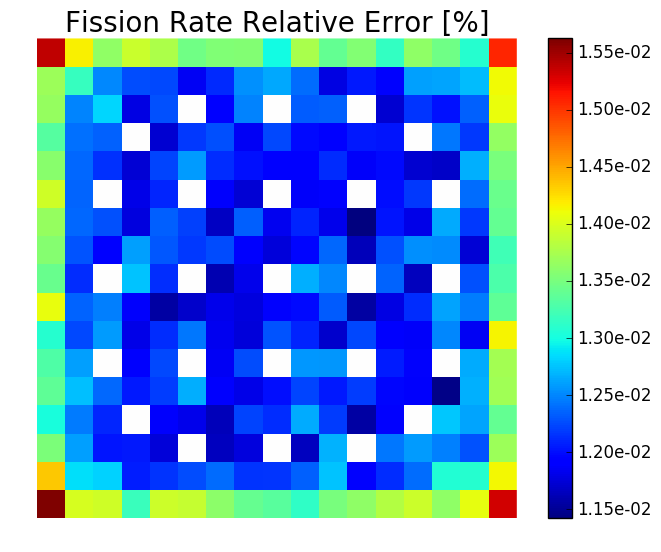
\includegraphics[width=\linewidth]{figures/benchmarks/fission-rates/fiss-rel-err-assm-16}
  \caption{}
  \label{fig:chap7-fiss-rate-rel-err-1.6-assm}
\end{subfigure}%
\caption[Fission rates for a 1.6\% enriched assembly]{Fission rates for a 1.6\% enriched assembly.}
\label{fig:chap7-fiss-rates-1.6-assm}
\end{figure}

\begin{figure}[h!]
\centering
\begin{subfigure}{0.44\textwidth}
  \centering
  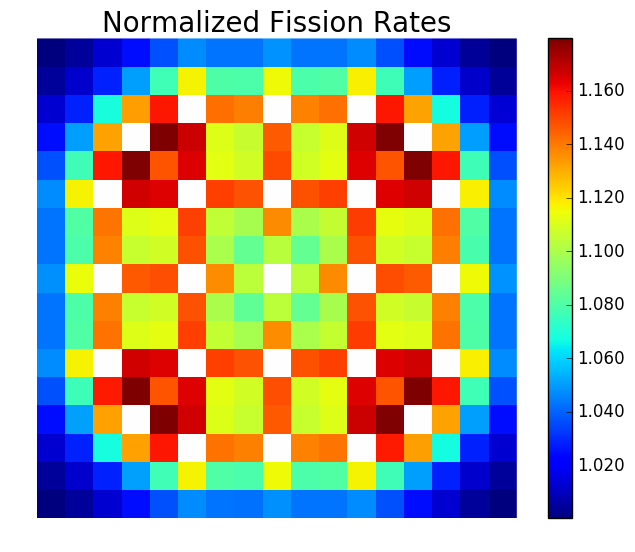
\includegraphics[width=\linewidth]{figures/benchmarks/fission-rates/fiss-mean-assm-31}
  \caption{}
  \label{fig:chap7-fiss-rate-mean-3.1-assm}
\end{subfigure}%
\begin{subfigure}{0.44\textwidth}
  \centering
  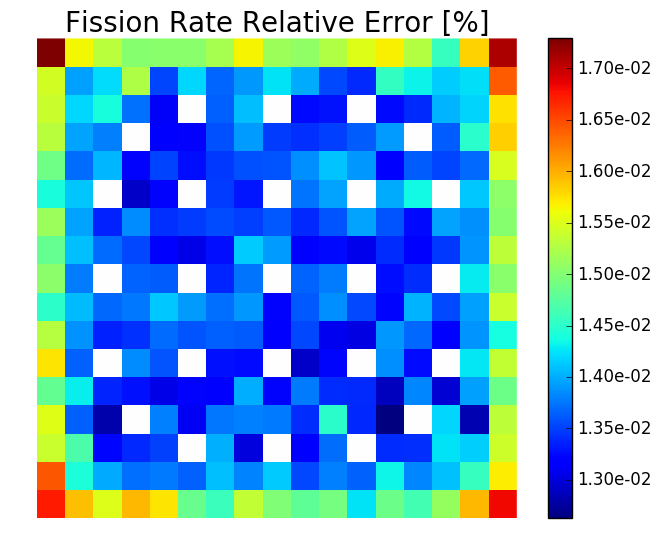
\includegraphics[width=\linewidth]{figures/benchmarks/fission-rates/fiss-rel-err-assm-31}
  \caption{}
  \label{fig:chap7-fiss-rate-rel-err-3.1-assm}
\end{subfigure}%
\caption[Fission rates for a 3.1\% enriched assembly]{Fission rates for a 3.1\% enriched assembly.}
\label{fig:chap7-fiss-rates-3.1-assm}
\end{figure}

\begin{figure}[h!]
\centering
\begin{subfigure}{0.44\textwidth}
  \centering
  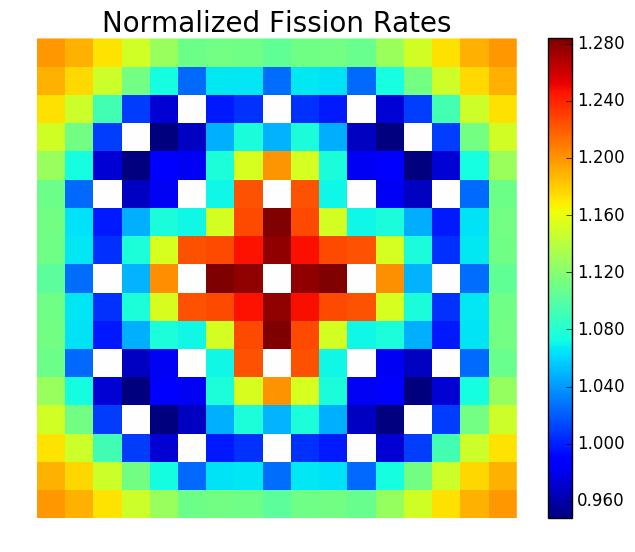
\includegraphics[width=\linewidth]{figures/benchmarks/fission-rates/fiss-mean-assm-31-20BPs}
  \caption{}
  \label{fig:chap7-fiss-rate-mean-3.1-20BAs-assm}
\end{subfigure}%
\begin{subfigure}{0.44\textwidth}
  \centering
  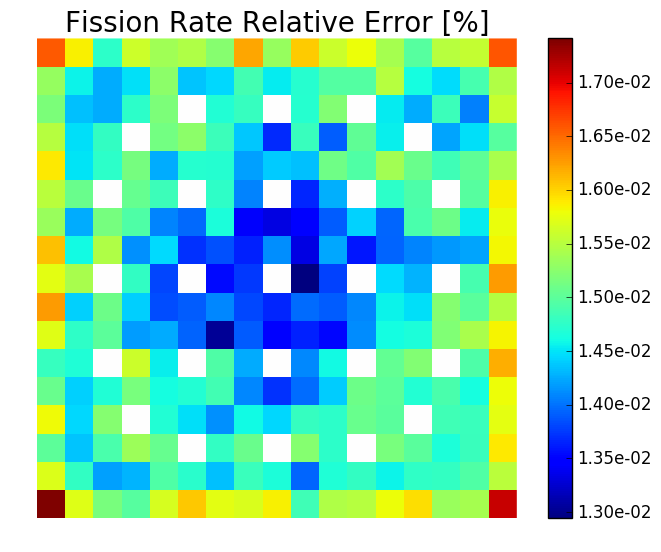
\includegraphics[width=\linewidth]{figures/benchmarks/fission-rates/fiss-rel-err-assm-31-20BPs}
  \caption{}
  \label{fig:chap7-fiss-rate-rel-err-3.1-20BAs-assm}
\end{subfigure}%
\caption[Fission rates for a 3.1\% enriched assembly with 20 BPs]{Fission rates for a 3.1\% enriched assembly with 20 \ac{BP}s.}
\label{fig:chap7-fiss-rates-3.1-assm-20BAs}
\end{figure}

\begin{figure}[h!]
\centering
\begin{subfigure}{0.44\textwidth}
  \centering
  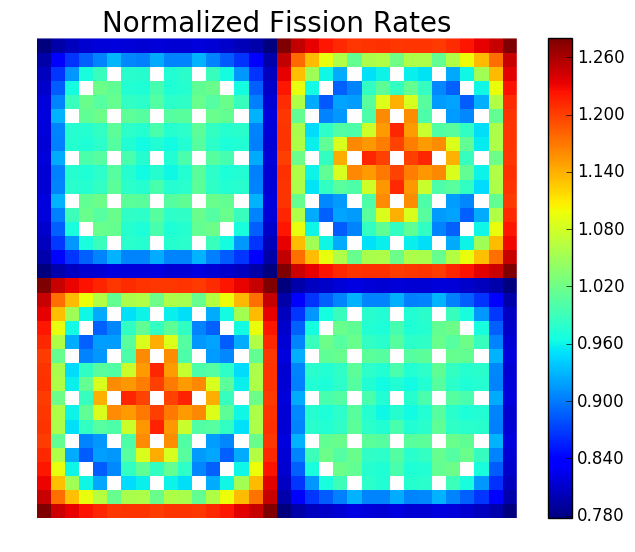
\includegraphics[width=\linewidth]{figures/benchmarks/fission-rates/fiss-mean-2x2}
  \caption{}
  \label{fig:chap7-fiss-rate-mean-2x2}
\end{subfigure}%
\begin{subfigure}{0.44\textwidth}
  \centering
  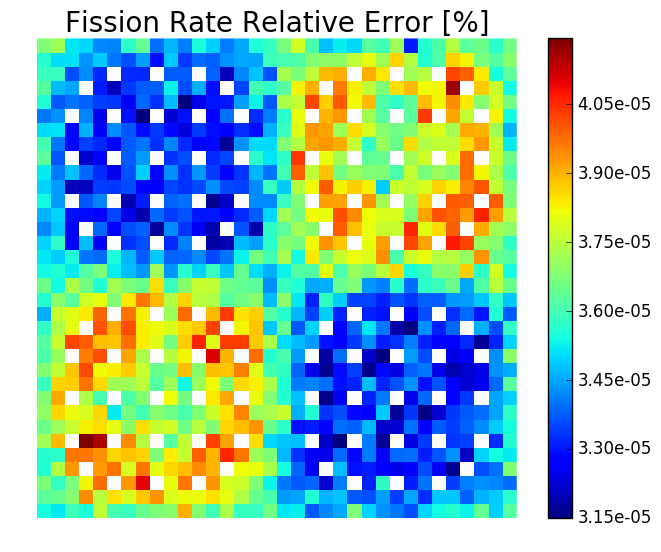
\includegraphics[width=\linewidth]{figures/benchmarks/fission-rates/fiss-rel-err-2x2}
  \caption{}
  \label{fig:chap7-fiss-rate-rel-err-2x2}
\end{subfigure}%
\caption[Fission rates for a 2$\times$2 colorset]{Fission rates for a 2$\times$2 colorset.}
\label{fig:chap7-fiss-rates-2x2}
\end{figure}

\begin{figure}[h!]
\centering
\begin{subfigure}{0.44\textwidth}
  \centering
  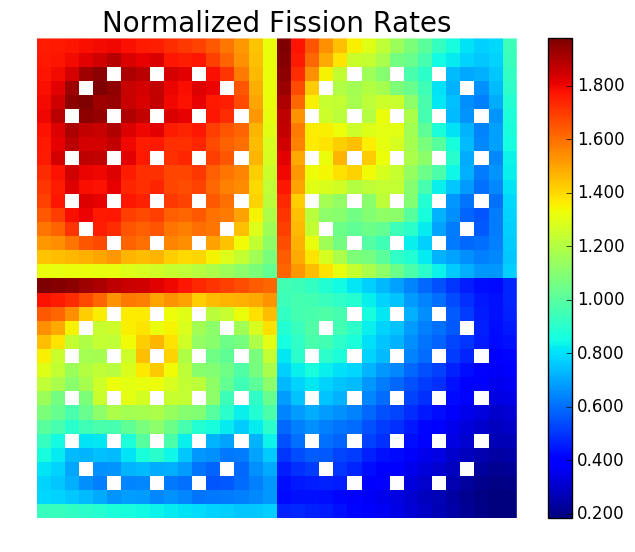
\includegraphics[width=\linewidth]{figures/benchmarks/fission-rates/fiss-mean-reflector}
  \caption{}
  \label{fig:chap7-fiss-rate-conv}
\end{subfigure}%
\begin{subfigure}{0.44\textwidth}
  \centering
  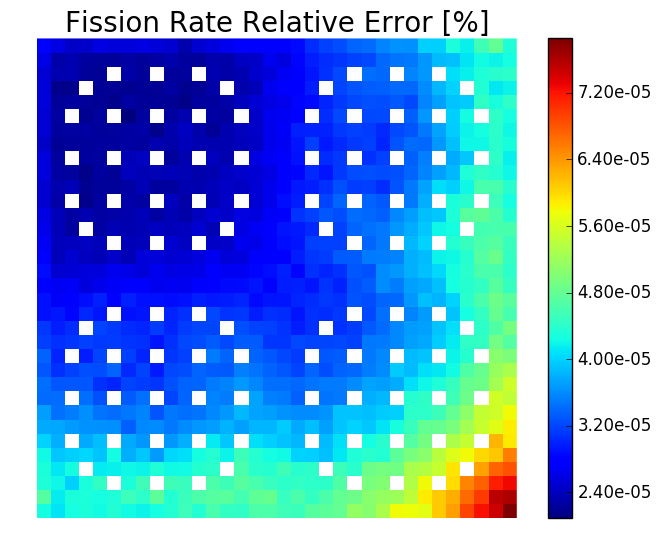
\includegraphics[width=\linewidth]{figures/benchmarks/fission-rates/fiss-rel-err-reflector}
  \caption{}
  \label{fig:chap7-fiss-rate-conv}
\end{subfigure}%
\caption[Fission rates for a 2$\times$2 colorset with a reflector]{Fission rates for a 2$\times$2 colorset with a reflector.}
\label{fig:chap7-fiss-rates-reflector}
\end{figure}

\begin{figure}[h!]
\centering
\begin{subfigure}{0.44\textwidth}
  \centering
  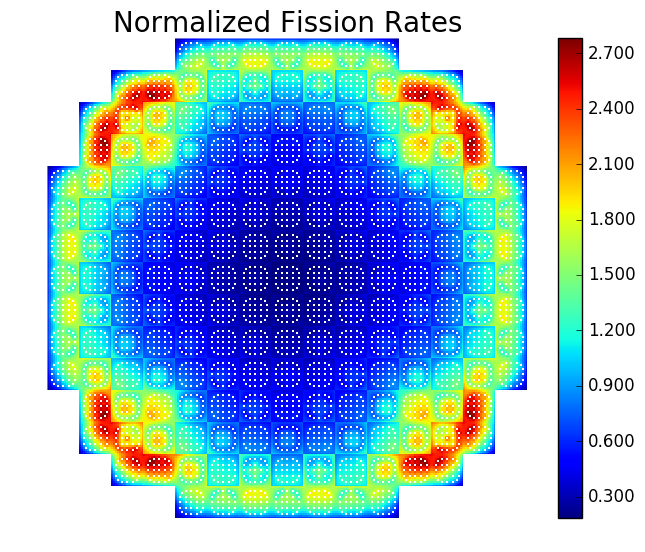
\includegraphics[width=\linewidth]{figures/benchmarks/fission-rates/fiss-mean-full-core}
  \caption{}
  \label{fig:chap7-fiss-rate-mean-full-core}
\end{subfigure}%
\begin{subfigure}{0.44\textwidth}
  \centering
  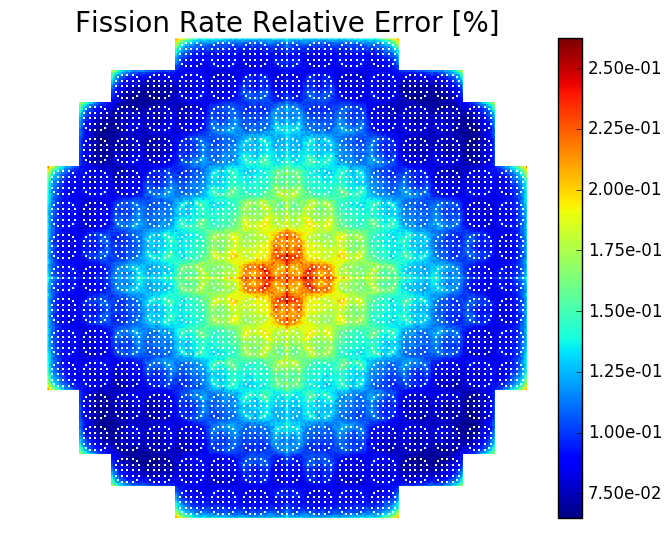
\includegraphics[width=\linewidth]{figures/benchmarks/fission-rates/fiss-rel-err-full-core}
  \caption{}
  \label{fig:chap7-fiss-rate-rel-err-full-core}
\end{subfigure}%
\caption[Fission rates for the full 2D BEAVRS core]{Fission rates for the 2D quarter core \ac{BEAVRS} model.}
\label{fig:chap7-fiss-rates-full-core}
\end{figure}

%\begin{figure}[h!]
%\centering
%\begin{subfigure}{\textwidth}
%  \centering
%  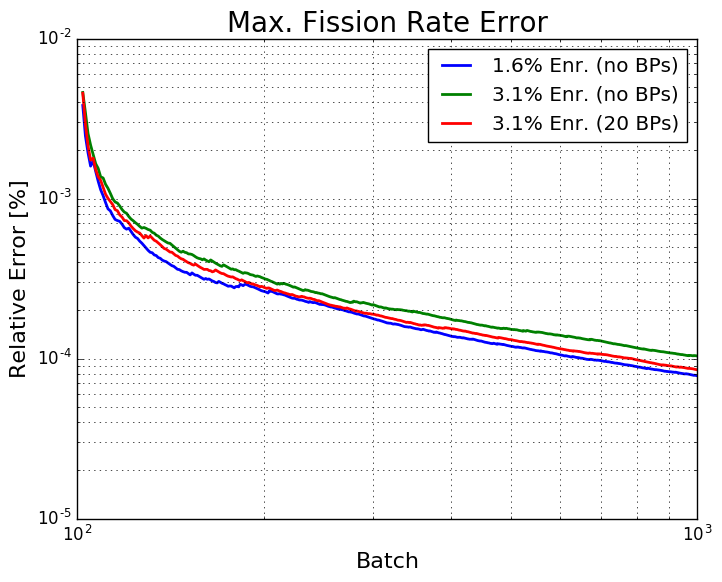
\includegraphics[width=0.8\linewidth]{figures/benchmarks/fission-rates/fiss-conv-max-assms}
%  \caption{}
%  \label{fig:chap7-fiss-rate-max-conv-max}
%\end{subfigure}
%\begin{subfigure}{\textwidth}
%  \centering
%  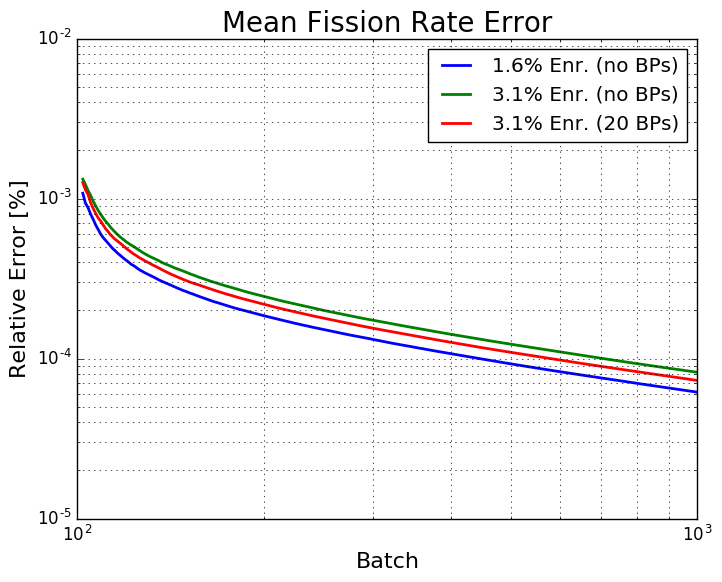
\includegraphics[width=0.8\linewidth]{figures/benchmarks/fission-rates/fiss-conv-mean-assms}
%  \caption{}
%  \label{fig:chap7-fiss-rate-max-conv-mean}
%\end{subfigure}
%\caption[Fission rate relative error convergence for BEAVRS geometries]{The maximum (a) and mean (b) fission rate relative error convergence for the six heterogeneous benchmark geometries.}
%\label{fig:chap7-fiss-rates-conv}
%\end{figure}

\clearpage

%%%%%%%%%%%%%%%%%%%%%%%%%%%%%%%%%%%%%%%%%%%%%
\subsection{U-238 Capture Rate Spatial Distributions}
\label{subsec:chap7-capture-rates}

The reference energy-integrated U-238 capture rate spatial distributions for each of the six benchmarks were computed using rectilinear, pin-wise tally meshes in OpenMC. The U-238 capture rates were volume-integrated across each fuel pin. The capture rates were normalized to the mean of all non-zero capture rates in each benchmark. The percent relative errors for the tallied capture rates was computed from the ratio of the sample standard deviation to the mean capture rate in each fuel pin. The capture rates for the quarter core \ac{BEAVRS} model were appropriately tiled to display the equivalent distribution across the quadrant symmetric full core.

The U-238 capture rate spatial distributions and percent relative errors for each of the six benchmarks are presented as heatmaps in Figs.~\Crefrange{fig:chap7-capt-rates-1.6-assm}{fig:chap7-capt-rates-full-core}. The capture rates in the instrument tubes, \acp{CRGT} and \acp{BP} are all zero and are illustrated in white. The color bars for each of the heatmaps range from the minimum non-zero capture rate to the maximum capture rate for all fuel pins in each benchmark geometry. The maximum relative error at the final 1000$^{\text{th}}$ batch is less than 0.5\% for all of the benchmarks. These reference U-238 capture rate spatial distributions are used to validate the OpenMOC simulations with \ac{MGXS} generated by from OpenMC throughout the following chapters.

%The batch-wise convergence rates of the capture rates is shown for the maximum and mean percent relative errors for each of the benchmarks in Fig.~\ref{fig:chap7-capt-rates-conv}.

The impacts of \acp{CRGT}, \acp{BP}, reflectors and vacuum \acp{BC} on the U-238 capture rates are similar to those observed for the fission rates, though there are some noticeable differences. For example, the U-238 capture rates in the individual fuel assemblies appear to be more sensitive than the fission rates to the spatial self-shielding induced by moderation in \acp{CRGT}. In addition, the U-238 capture rates peak in the 1.6\% enriched fuel assemblies in the 2$\times$2 colorset without a reflector (Fig.~\ref{fig:chap7-capt-rate-rel-err-2x2}), while the fission rates peak in the 3.1\% enriched fuel assemblies (Fig.~\ref{fig:chap7-fiss-rate-rel-err-2x2}). The key reason for this is that there is a higher concentration of U-238 in the 1.6\% enriched fuel than the 3.1\% enriched fuel, which leads to a lower ratio of fission to U-238 capture rates. In addition, the U-238 capture rates in the reflected 2$\times$2 benchmark (Fig.~\ref{fig:chap7-capt-rates-reflector}) are more smoothly varying at the inter-assembly interface than the fission rates (Fig.~\ref{fig:chap7-fiss-rates-reflector}).

\begin{figure}[h!]
\centering
\begin{subfigure}{0.44\textwidth}
  \centering
  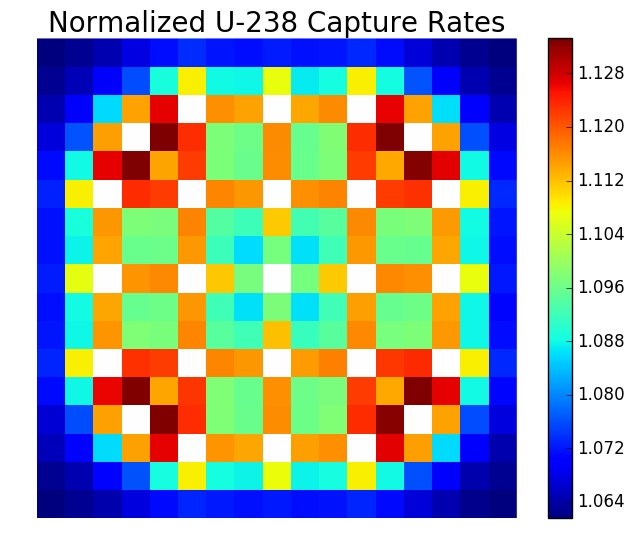
\includegraphics[width=\linewidth]{figures/benchmarks/capture-rates/capt-mean-assm-16}
  \caption{}
  \label{fig:chap7-capt-rate-mean-1.6-assm}
\end{subfigure}%
\begin{subfigure}{0.44\textwidth}
  \centering
  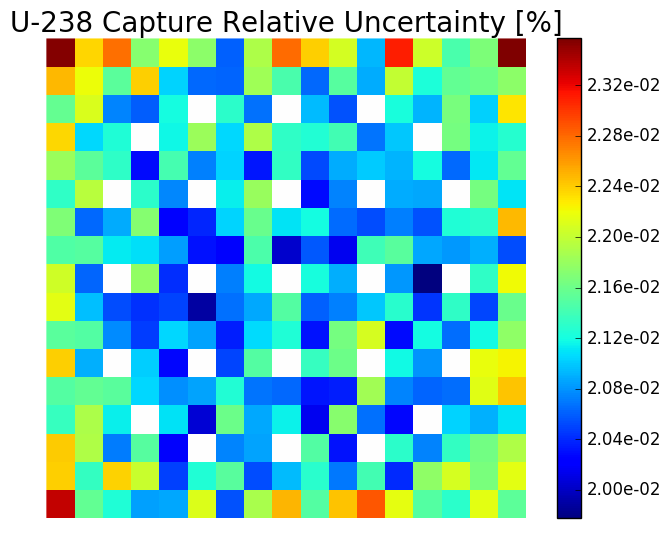
\includegraphics[width=\linewidth]{figures/benchmarks/capture-rates/capt-rel-err-assm-16}
  \caption{}
  \label{fig:chap7-capt-rate-rel-err-1.6-assm}
\end{subfigure}%
\caption[U-238 capture rates for a 1.6\% enriched assembly]{U-238 capture rates for a 1.6\% enriched assembly.}
\label{fig:chap7-capt-rates-1.6-assm}
\end{figure}

\begin{figure}[h!]
\centering
\begin{subfigure}{0.44\textwidth}
  \centering
  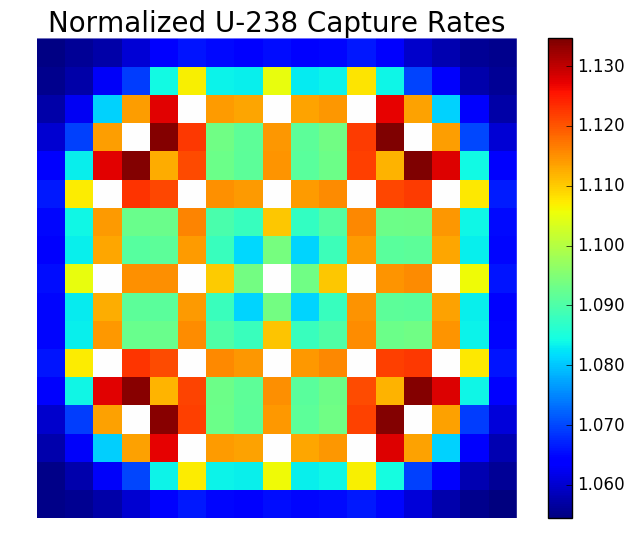
\includegraphics[width=\linewidth]{figures/benchmarks/capture-rates/capt-mean-assm-31}
  \caption{}
  \label{fig:chap7-capt-rate-mean-3.1-assm}
\end{subfigure}%
\begin{subfigure}{0.44\textwidth}
  \centering
  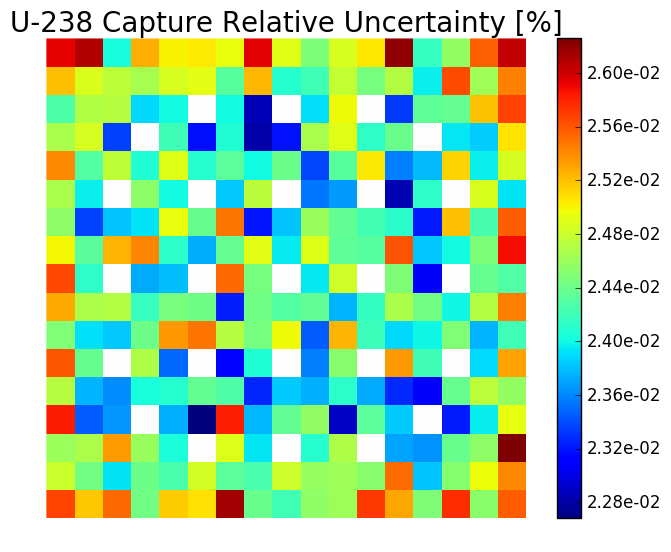
\includegraphics[width=\linewidth]{figures/benchmarks/capture-rates/capt-rel-err-assm-31}
  \caption{}
  \label{fig:chap7-capt-rate-rel-err-3.1-assm}
\end{subfigure}%
\caption[U-238 capture rates for a 3.1\% enriched assembly]{U-238 capture rates for a 3.1\% enriched assembly.}
\label{fig:chap7-capt-rates-3.1-assm}
\end{figure}

\begin{figure}[h!]
\centering
\begin{subfigure}{0.44\textwidth}
  \centering
  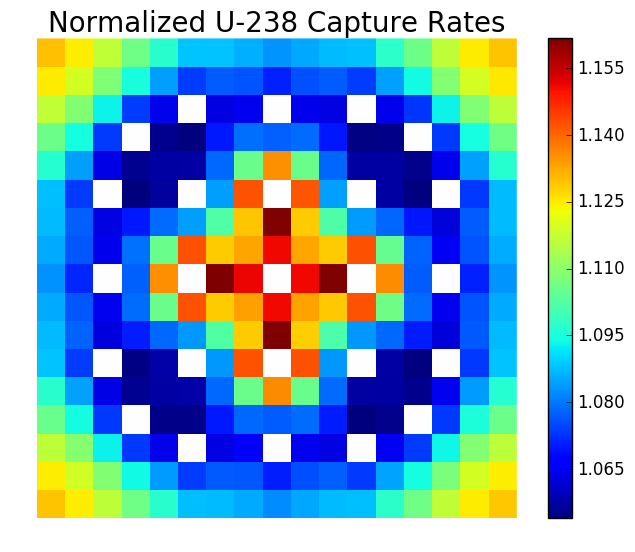
\includegraphics[width=\linewidth]{figures/benchmarks/capture-rates/capt-mean-assm-31-20BPs}
  \caption{}
  \label{fig:chap7-capt-rate-mean-3.1-20BAs-assm}
\end{subfigure}%
\begin{subfigure}{0.44\textwidth}
  \centering
  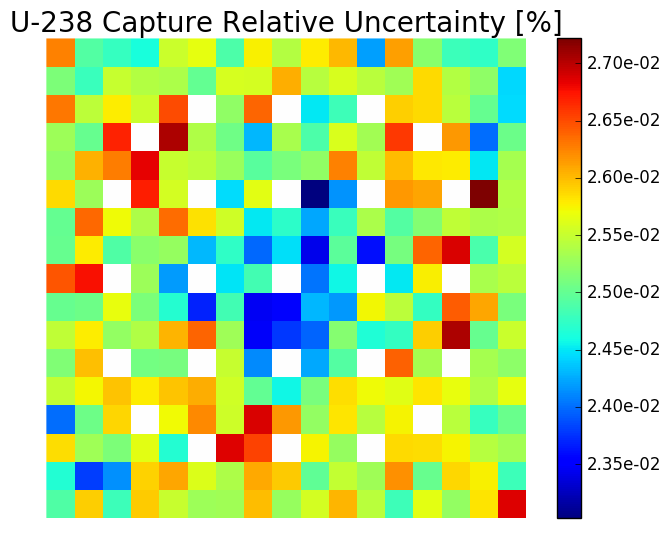
\includegraphics[width=\linewidth]{figures/benchmarks/capture-rates/capt-rel-err-assm-31-20BPs}
  \caption{}
  \label{fig:chap7-capt-rate-rel-err-3.1-20BAs-assm}
\end{subfigure}%
\caption[U-238 capture rates for a 3.1\% enriched assembly with 20 BPs]{U-238 capture rates for a 3.1\% enriched assembly with 20 \ac{BP}s.}
\label{fig:chap7-capt-rates-3.1-assm-20BAs}
\end{figure}

\begin{figure}[h!]
\centering
\begin{subfigure}{0.44\textwidth}
  \centering
  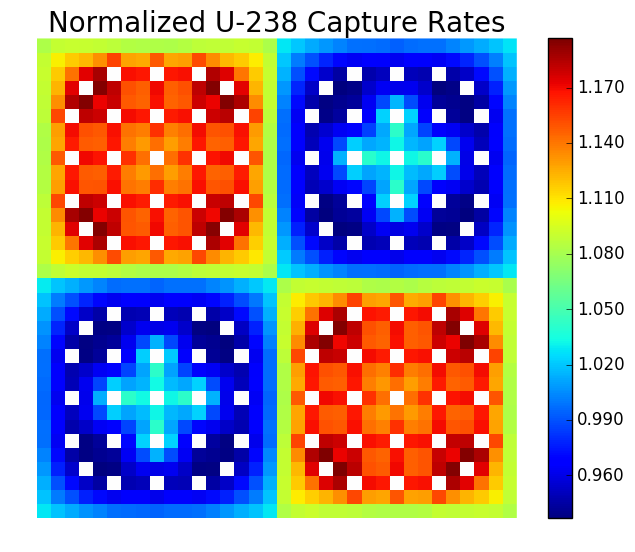
\includegraphics[width=\linewidth]{figures/benchmarks/capture-rates/capt-mean-2x2}
  \caption{}
  \label{fig:chap7-capt-rate-mean-2x2}
\end{subfigure}%
\begin{subfigure}{0.44\textwidth}
  \centering
  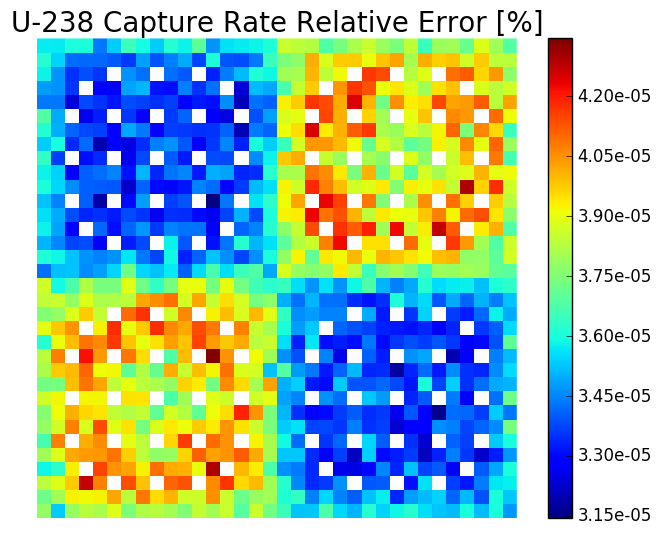
\includegraphics[width=\linewidth]{figures/benchmarks/capture-rates/capt-rel-err-2x2}
  \caption{}
  \label{fig:chap7-capt-rate-rel-err-2x2}
\end{subfigure}%
\caption[U-238 capture rates for a 2$\times$2 colorset]{U-238 capture rates for a 2$\times$2 colorset.}
\label{fig:chap7-capt-rates-2x2}
\end{figure}

\begin{figure}[h!]
\centering
\begin{subfigure}{0.44\textwidth}
  \centering
  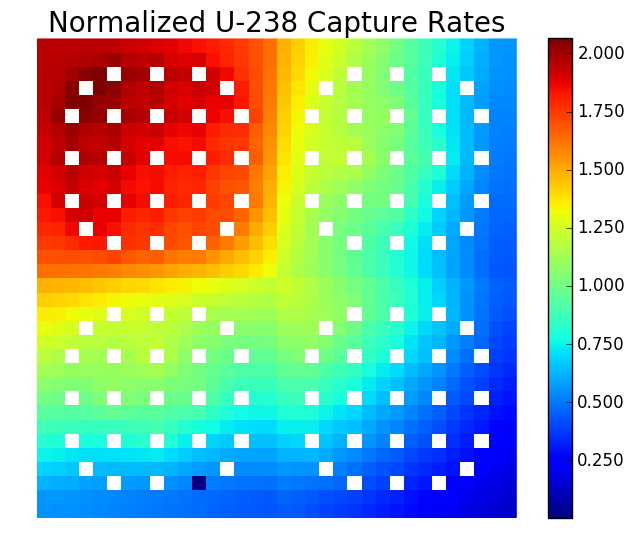
\includegraphics[width=\linewidth]{figures/benchmarks/capture-rates/capt-mean-reflector}
  \caption{}
  \label{fig:chap7-capt-rate-mean-reflector}
\end{subfigure}%
\begin{subfigure}{0.44\textwidth}
  \centering
  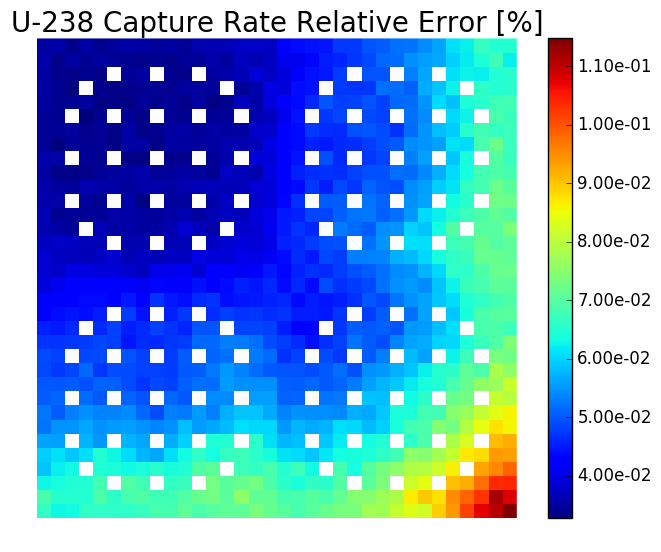
\includegraphics[width=\linewidth]{figures/benchmarks/capture-rates/capt-rel-err-reflector}
  \caption{}
  \label{fig:chap7-capt-rate-rel-err-reflector}
\end{subfigure}%
\caption[U-238 capture rates for a 2$\times$2 colorset with a reflector]{U-238 capture rates for a 2$\times$2 colorset with a reflector.}
\label{fig:chap7-capt-rates-reflector}
\end{figure}

\begin{figure}[h!]
\centering
\begin{subfigure}{0.44\textwidth}
  \centering
  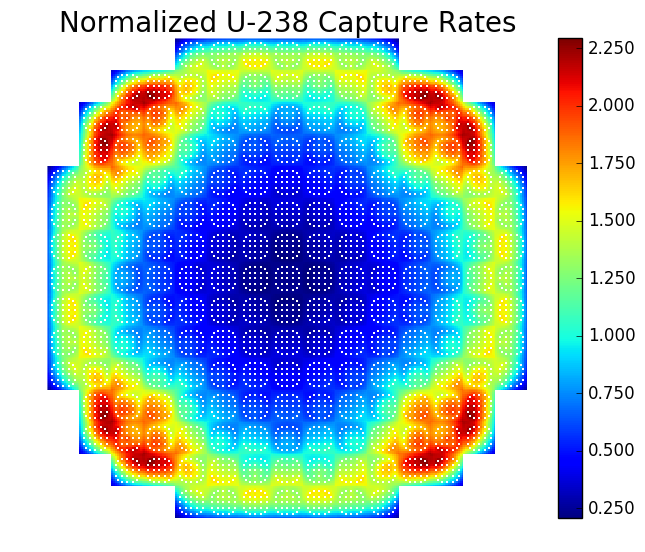
\includegraphics[width=\linewidth]{figures/benchmarks/capture-rates/capt-mean-full-core}
  \caption{}
  \label{fig:chap7-capt-rate-mean-full-core}
\end{subfigure}%
\begin{subfigure}{0.44\textwidth}
  \centering
  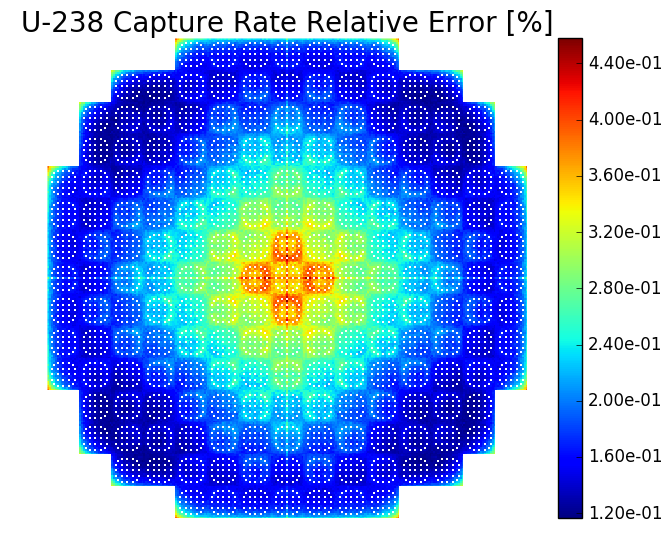
\includegraphics[width=\linewidth]{figures/benchmarks/capture-rates/capt-rel-err-full-core}
  \caption{}
  \label{fig:chap7-capt-rate-rel-err-full-core}
\end{subfigure}%
\caption[U-238 capture rates for the full 2D BEAVRS core]{U-238 capture rates for the 2D quarter core \ac{BEAVRS} model.}
\label{fig:chap7-capt-rates-full-core}
\end{figure}

Similar to the fission rates, the U-238 capture rate distribution for the quarter core \ac{BEAVRS} model is highly skewed due to the isotropic in lab scattering approximation. This can be seen from comparison of Fig.~\ref{fig:chap7-capt-rate-mean-full-core} with the true capture rate distribution calculated with normal anisotropic scattering in Fig.~\ref{fig:benchmarks-beavrs-capt-aniso}. Like fission, the U-238 capture distribution is highly sensitive to anisotropic scattering due to radial leakage out of the core, and is more peaked near the corner reflectors when the isotropic approximation is made. Although isotropic scattering is unphysical, it allows direct comparisons of OpenMC and OpenMOC results in latter chapters to quantify the impact of various approaches to spatially homogenize \ac{MGXS} without conflicting effects due to the isotropic scattering model used in OpenMOC.

%\begin{figure}[h!]
%\centering
%\begin{subfigure}{\textwidth}
%  \centering
%  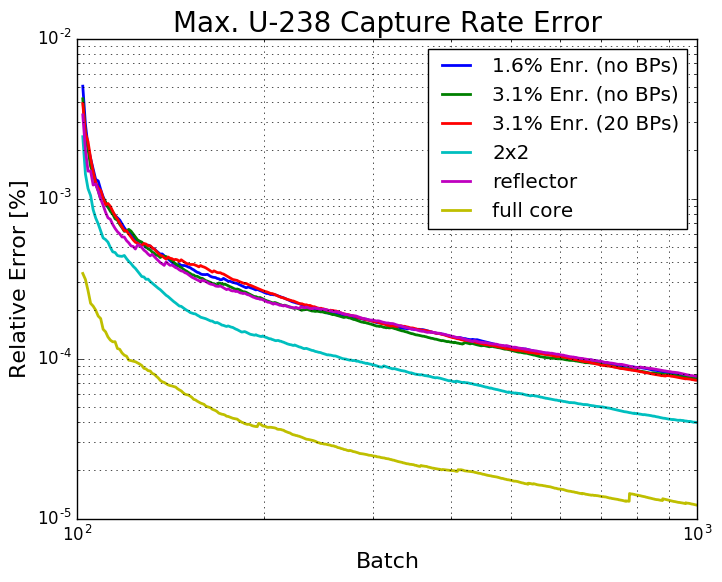
\includegraphics[width=0.8\linewidth]{figures/benchmarks/capture-rates/capt-conv-max-assms}
%  \caption{}
%  \label{fig:chap7-capt-rate-max-conv}
%\end{subfigure}
%\begin{subfigure}{\textwidth}
%  \centering
%  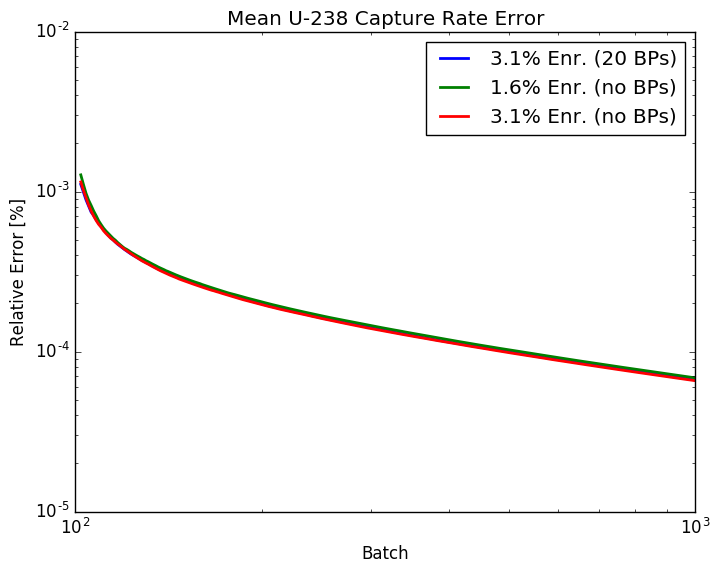
\includegraphics[width=0.8\linewidth]{figures/benchmarks/capture-rates/capt-conv-mean-assms}
%  \caption{}
%  \label{fig:chap7-capt-rate-max-conv}
%\end{subfigure}
%\caption[U-238 capture rate relative error convergence for BEAVRS geometries]{The maximum (a) and mean (b) U-238 capture rate percent relative error convergence for the six heterogeneous benchmark geometries.}
%\label{fig:chap7-capt-rates-conv}
%\end{figure}

%\clearpage

\vfill
\begin{highlightsbox}[frametitle=Highlights]
\begin{itemize}
  \item A series of six 2D heterogeneous benchmark models were derived from the full core \ac{BEAVRS} model to explore spatial self-shielding effects on \ac{MGXS}.
  \item The benchmarks include individual fuel assemblies with different \ac{CRGT} and \ac{BP} configurations, 2$\times$2 fuel assembly colorsets with and without a water reflector, and the quarter core \ac{BEAVRS} model.
  \item The Shannon entropy was computed to determine the number of inactive batches needed when modeling each benchmark with OpenMC.
  \item Reference results for the eigenvalues, pin-wise fission rates and pin-wise U-238 capture rates were computed using OpenMC.
  \item The benchmarks and reference results are used in the following chapters to validate the use of statistical clustering methods to capture spatial self-shielding effects in \ac{MGXS} generated by OpenMC for OpenMOC.
\end{itemize}
\end{highlightsbox}
\vfill